% Beamer Presentation and Lecture Note Template
% Version 0.1
% by Paul Vesey

%%%%%%%%%%%%%%%%%%%%%%%%%%%%%%%%%%%%%
% Switch between these for presentation
% and A4 Lecture Notes
%\documentclass[ignorenonframetext,red]{beamer}     % use this for presentations and slide handouts
%\documentclass[ignorenonframetext]{beamer}     % use this for presentations and slide handouts
%\documentclass[a4paper]{article}     % use this to print the notes

%\documentclass{beamer}

%%%%%%%%%%%%%%%%%%%%%%%%%%%%%%%%%%%%%%%%
% Turn off all of these for A4 Notes
%
\mode<presentation> {
%\usetheme{lankton-keynote} % Seperate Download
%\usetheme{Madrid}
\usetheme{Antibes}
\setbeamercovered{invisible}
\setbeamertemplate{navigation symbols}{} 
}

%%\mode<presentation>{}



%%%%%%%%%%%%%%%%%%%%%%%%%%%%%%%%%%%%%%%%%%
%%%%%%%%%%%%%%%%%%%%%%%%%%%%%%%%%%%%%%%%%%

\usepackage{eurosym}
\usepackage{graphicx}
\usepackage{wasysym}
\usepackage{listings}
\usepackage{pxfonts}
\usepackage{verbatim}
\usepackage{color}
\usepackage{xcolor}
\usepackage{wrapfig}
\usepackage{hyperref}
\usepackage[nomain, xindy, toc, acronym]{glossaries}

%\newglossaryentry{html}
%{ name=HTML, description={Hypertext Markup Language is the backbone of webpages.  Static pages are simply served up by the webserver on request.  Dynamic pages are created and returned by the webserver on the fly.},
%}



%\newglossaryentry{css}
%{  name=CSS, description={Cascading Style Sheets are a way to apply styling to web-pages. It can be inline, or through an external file.  An external file is the best approach.},
%}




\newglossaryentry{Linux}
{
  name=Linux,
  description={is a generic term referring to the family of Unix-like
               computer operating systems that use the Linux kernel},
  plural=Linuces
}

\newglossaryentry{DOM1}
{
  name=DOM Level 1,
  description={The DOM Level 1 specification is separated into two parts: Core and HTML. The Core DOM Level 1 section provides a low-level set of fundamental interfaces that can represent any structured document, as well as defining extended interfaces for representing an XML document.}
}

\newglossaryentry{Apache}
{
  name=Apache,
  description={Open-source web server developed by the Apache Foundation.  One of the most widely used webservers on the planet.}
}

\newglossaryentry{JS}
{
  name=JavaScript,
  description={Scripting Language often included in web pages.  Requires an interpreter in the browser.}
}



\newglossaryentry{MySQL}{name=MySQL,
description={database engine by Oracle}}


\newglossaryentry{PDO}{name=PDO,
description={php Data Objects.  A lightweight database abstraction layer for php}}

\newglossaryentry{zxing}{name=ZXing,
description={pronounced Zebra Crossing, ZXing is an open-source bar-code scanner project.  ZXing can read standard bar-codes and QR codes}}

\newglossaryentry{QR}{name=QR,
description={Quick Response Code. A form of two dimensional machine readable image similar to a traditional bar code}}


\newglossaryentry{JavaScript}{name=JavaScript,
description={An interpreted computer language in widespread use in web applications}}


\newglossaryentry{php}{name=php,
description={php Hypertext Preprocessor. An interpreted computer language in widespread use on web servers}}



\newglossaryentry{Android}{name=Android,
description={A Linux based operating system for Smartphones and tablet computers}}



\newglossaryentry{ProGuard}{name=ProGuard,
description={A tool for optimizing and obfuscating compiled Android Apps}}

\newacronym{lvm}{LVM}{Logical Volume Manager}
\newacronym{html}{HTML}{Hypertext Markup Language}
\newacronym{xml}{XML}{Extensible Markup Language}
\newacronym{css}{CSS}{Cascading Style Sheets}
\newacronym{dom}{DOM}{Document Object Model}
\newacronym{url}{URL}{Uniform Resource Locator}
\newacronym{SQL}{SQL}{Structured Query Language}
\newacronym{oop}{OOP}{Object Orientated Programming}
\newacronym{RFID}{RFID}{Radio Frequency Identification}
\newacronym{VLE}{VLE}{Virtual Learning Environment}
\newacronym{api}{API}{Application Program Interface}
\newacronym{https}{HTTPS}{Hypertext Transfer Protocol Secure}
\newacronym{tcpip}{TCP/IP}{Transmission Control Protocol / Internet Protocol}
\newacronym{uml}{UML}{Unified Modeling Language}
\newacronym{lamp}{LAMP}{Linux, Apache, MySQL, php}
\newacronym{AMP}{LAMP}{Linux, Apache, MySQL, php}
\newacronym{ftp}{FTP}{File Transfer Protocol}
\newacronym{sdk}{SDK}{Software Development Kit}
\newacronym{lcd}{LCD}{Liquid Crystal Display}
\newacronym{ajax}{AJAX}{Asynchronous Javascript and XML}
\newacronym{IDE}{IDE}{Integrated Development Environment}
\newacronym{IE}{IE}{Microsoft Internet Explorer}
\newacronym{WiFi}{WiFi}{Wireless Local Area Network}

\makeglossaries{}
\usepackage[xindy]{imakeidx}
\makeindex




%%%%%%%%%%%%%%%%%%%%%%%%%%%%%%%%%%%%%%%%%%%%%%%%%%%%%%
%%%%%%%%%%%%%%%%%%%%%%%%%%%%%%%%%%%%%%%%%%%%%%%%%%%%%%
%
%THIS IS FOR PRINTING SLIDE HANDOUTS
%\usepackage{pgfpages}
%\pgfpagesuselayout{2 on 1}[a4paper,border shrink=5mm]

%%%%%%%%%%%%%%%%%%%%%%%%%%%%%%%%%%%%%%%%%%%%%%%%%%%%%%%
%%%%%%%%%%%%%%%%%%%%%%%%%%%%%%%%%%%%%%%%%%%%%%%%%%%%%%
%
%THIS IS FOR PRINTING A4 NOTES
%
%\usepackage{beamerarticle}    % Turn this on for A4 notes

%%%%%%%%%%%%%%%%%%%%%%%%%%%%%%%%%%%%%%%%%%%%%%%%%%%%%%

%\renewcommand\verbatim@font{\color{red}\normalfont\ttfamily}




%\usepackage{bm} 
% For typesetting bold math (not \mathbold)
%\logo{\includegraphics[height=0.6cm]{yourlogo.eps}}
%
\title[Advanced Graphics \& Visualisation]{Advanced Graphics \& Visualisation}
%
\author{Paul Vesey}
\institute[LIT]
{
Limerick Institute of Technology \\
\medskip
{\emph{paul.vesey@lit.ie}}
}
\date{2017-2018}
% \today will show current date. 
% Alternatively, you can specify a date.

\begin{document}
%

%\lstset{language=C++, frame=single}

\lstset{language=HTML,
				basicstyle=\small,
				breaklines=true,
        numbers=left,
        numberstyle=\tiny,
        showstringspaces=false,
        aboveskip=-20pt,
        frame=leftline
        }



\tableofcontents
\newpage



\begin{frame}
\titlepage
\end{frame}\begin{center}\line(1,0){250}\end{center}
%
%


\section{Introduction}




\begin{frame}
\frametitle{About me}
\begin{itemize}
	\item Paul Vesey
	\item 13B09
	\item email is best
\end{itemize}

\end{frame}
\begin{center}\line(1,0){250}\end{center}







\begin{frame}
\frametitle{The course in a nutshell}
\begin{itemize}
	\item Technology
	\item Composition \& Image Creation
	\item Digital Images
	\item Digital Video \& Game Engine
\end{itemize}
\end{frame}\begin{center}\line(1,0){250}\end{center}


 
 \begin{frame}
\frametitle{Learning Outcomes}
On successful completion of this module the learner will/should be able to\ldots
\begin{enumerate}
	\item Understand the hardware and software technology requirements for advanced visualization.
	\item Understand image composition, DOF, color, hue, and other image characteristics.
	\item Develop and critique photo-realistic rendered images of building interior and exteriors.
	\item Develop professional level video animations of virtual environments.
\end{enumerate}
\end{frame}
\begin{center}\line(1,0){250}\end{center}



\begin{frame}
\frametitle{Indicative Syllabus \hfill\hfill Technology}

\begin{itemize}
	\item Hardware and Software
	\item Ray Tracing, Graphics Processors, Memory, Distributed Processing
	\item Rendering Engines and Methods
	\item Compression Technologies and File Types
\end{itemize}
\end{frame}
\begin{center}\line(1,0){250}\end{center}



\begin{frame}
\frametitle{Indicative Syllabus \hfill\hfill Composition \& Image Creation}

\begin{itemize}
	\item Pattern, Symmetry, Texture, Depth of Field, Lines
	\item Lens Characteristics, Lighting Characteristics, 
	\item Dominance \& Subordination, Unity, Coherence, Positive \& Negative Space
	\item Balance, Shutter, Aperture, Light Measurement, Focus
\end{itemize}
\end{frame}
\begin{center}\line(1,0){250}\end{center}


\begin{frame}
\frametitle{Indicative Syllabus \hfill\hfill Digital Images}

\begin{itemize}
	\item Material Creation, Editing and Applicaiton
	\item Texture Creation, Editing and Application
	\item Cameras, Simulated Lighting, Artistic Lighting
	\item Post Processing, RPC Content
\end{itemize}
\end{frame}
\begin{center}\line(1,0){250}\end{center}


\begin{frame}
\frametitle{Indicative Syllabus \hfill\hfill Digital Video \& Game Engine}

\begin{itemize}
	\item Animation and Production Process
	\item Video Editing, Effects, and Audio
	\item Game Environments, Asset Creation and Management
	\item Controller Technologies
\end{itemize}
\end{frame}
\begin{center}\line(1,0){250}\end{center}






\begin{frame}
\frametitle{Assessment}
\textbf{100\% Continuous Assessment}
\begin{table}[htp]
	\centering
		\begin{tabular}{|l|l|}
			\hline
			\textbf{Assessment} & \textbf{Proportion} \\
			\hline
			Collection of photo-realistic images &		35\% \\
			5 minute animated video 						&   	35\% 			\\
			End of Year Integrated Project (Studio)  & 30\% 		\\
			\hline
		\end{tabular}
		\label{tab:Assessments}
\end{table}
\begin{itemize}
	\item The End of Year Project will be integrated into the studio project deliverables\\
	\item There will be numerous application studies throughout the year that will count towards each assessment.
\end{itemize}
\end{frame}
\begin{center}\line(1,0){250}\end{center}





\begin{table}[htp]
	\centering
		\scalebox{1.0}{
		\begin{tabular}{|c|r|l|}
			\hline
			\textbf{Week} & \textbf{Date } & \textbf{Activity}	\\
			\hline
			1		&	15/9	& Intro / Revit Revision				\\	
			2		&	22/9	& Revit Revision 								\\	
			3		&	29/9	& Revit	to Unity 3D							\\	
			4		&	6/10	& Unity 3D Workflow							\\	
			5		&	13/10	& Unity 3D Terrain 							\\	
			6		&	20/10	& Unity 3D Controllers					\\	
			7		&	26/10	& Bank Holiday									\\	
			8		&	3/11	& 								\\	
			9 	&	10/11	& 								\\	
			10	&	17/11	& 								\\
			11	&	24/11	& 								\\
			12	&	1/12	& 	\\
			
			
			13	&	8/12	& Christmas Exams								\\
					& 			& \textbf{Christmas Break}			\\
			14	& 5/1		&		\\
			15	& 12/1	&				\\
			16	& 19/1	&					\\
			17	& 26/1	&							\\										
			18	& 2/2		&							\\
			19	& 9/2		&	(Float)												\\
			20	& 16/2	&	 	\\
			21	& 23/2	&												\\										
			22	& 2/3		&										\\
			23	& 9/3		&											\\									
			24	& 16/3	&											\\
			25	& 23/3	&											\\										
				  & 			& \textbf{Easter Break}					\\
			26	& 13/4	&	EoY Project Support						\\
			27	& 20/4	&	EoY Project Support						\\									
			28	& 27/4	&	Presentations									\\
				  & 4/5		& Revision/Exam Week 						\\			
			\hline
		\end{tabular}}
				\label{tab:LessonPlanLong}
\end{table}




\section{Image Composition and Critique}



\begin{frame}
\frametitle{Composition}
\begin{itemize}
	\item Images should tell a story, engage the viewer, or elicit an emotional response.
	\item Images of interior design should do the same.
	\item ID images tend to fall into the documentary variety; there is no reason why ID images cannot be as engaging and exciting as other schools.
\end{itemize}
\end{frame}
\begin{center}\line(1,0){250}\end{center}


\begin{frame}
\frametitle{Emotion}
\begin{figure}
	\centering
		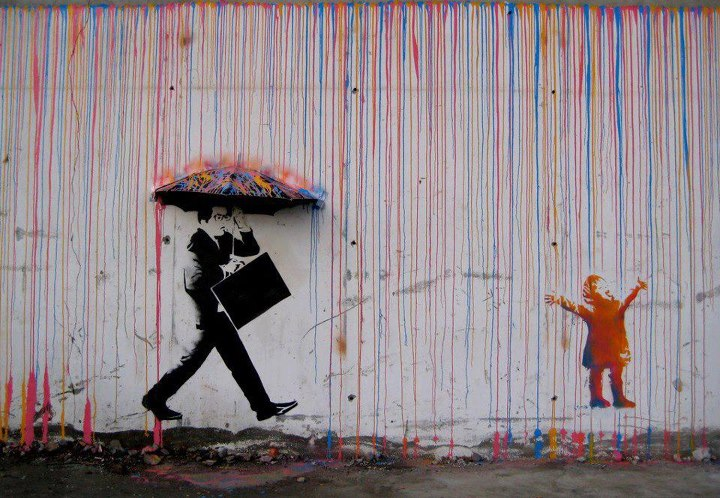
\includegraphics[width=8cm]{img/candc/2091078908.jpg}
	\caption{CMYK - skurktur}
	\label{fig:CMYK}
\end{figure}
\end{frame}
\begin{center}\line(1,0){250}\end{center}


\begin{frame}
\frametitle{Emotion}
\begin{figure}
	\centering
		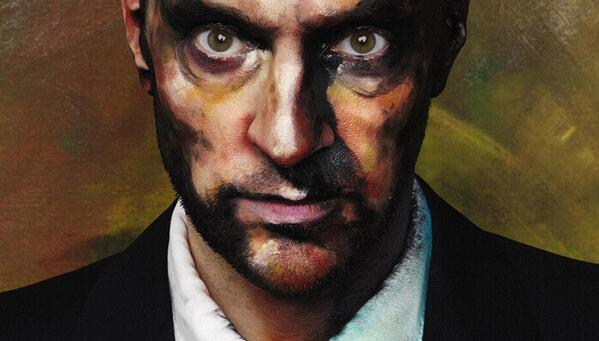
\includegraphics[height=6cm]{img/candc/DERREN-BROWN.jpg}
	\caption{Derren Brown}
	\label{fig:DerrenBrown}
\end{figure}
\end{frame}
\begin{center}\line(1,0){250}\end{center}



\begin{frame}
\frametitle{Emotion}
\begin{figure}
	\centering
		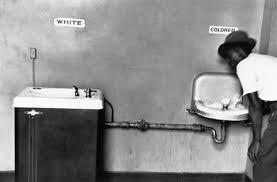
\includegraphics[height=6cm]{img/candc/whitesNonWhites.jpg}
	\caption{Elliott Erwitt - North Carolina in 1950}
	\label{fig:ElliottErwittNC}
\end{figure}
\end{frame}
\begin{center}\line(1,0){250}\end{center}





\begin{frame}
\frametitle{Tell a Story or Capture a Moment}
\begin{figure}
	\centering
		\includegraphics[height=6cm]{img/candc/18-Raphael-Paintings.jpg}
	\caption{Raphael - The Entombment (1508)}
	\label{fig:RaphaelEntombment}
\end{figure}
\end{frame}
\begin{center}\line(1,0){250}\end{center}




\begin{frame}
\frametitle{Tell a Story or Capture a Moment}
\begin{figure}
	\centering
		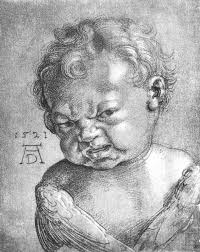
\includegraphics[height=6cm]{img/candc/DurerAngelBoy.jpg}
	\caption{Albrecht Durer - Weeping Angel boy, 1521}
	\label{fig:DurerAngelBoy}
\end{figure}
\end{frame}
\begin{center}\line(1,0){250}\end{center}




\begin{frame}
\frametitle{Tell a Story or Capture a Moment}
\begin{figure}
	\centering
		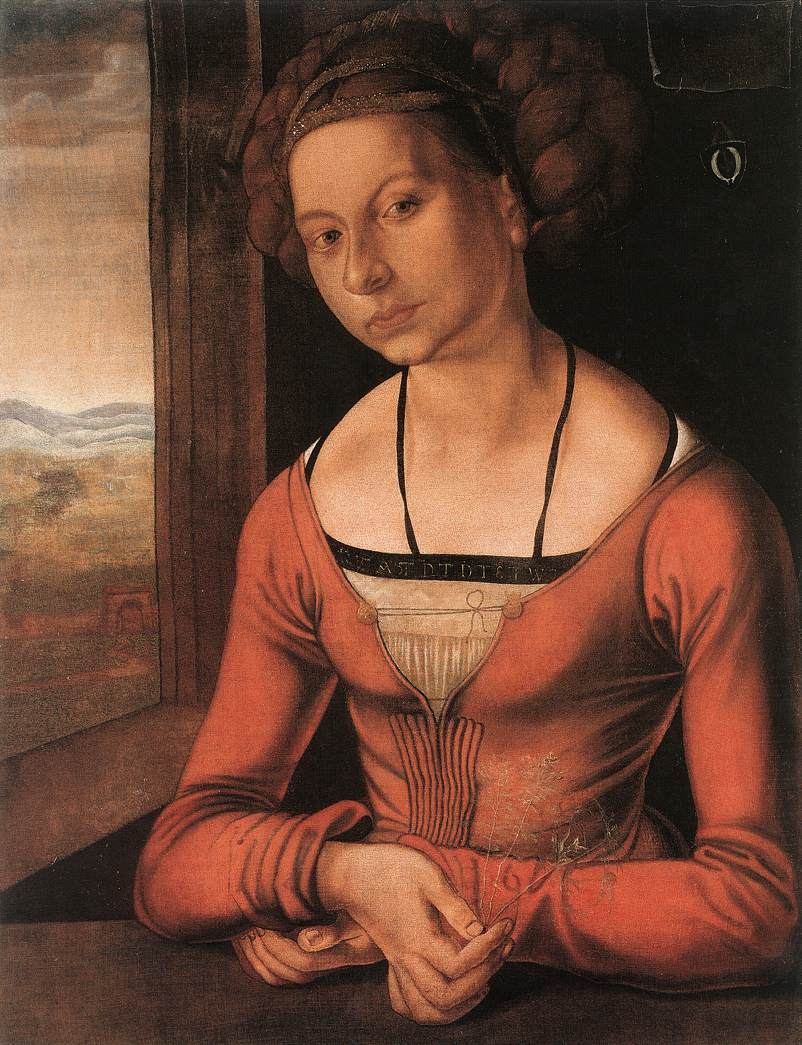
\includegraphics[height=6cm]{img/candc/Durerfurleger.jpg}
	\caption{Albrecht Durer - Portrait of a Young Furleger}
	\label{fig:DurerYoungFurleger}
\end{figure}
\end{frame}
\begin{center}\line(1,0){250}\end{center}




\begin{frame}
\frametitle{Tell a Story or Capture a Moment}
\begin{figure}
	\centering
		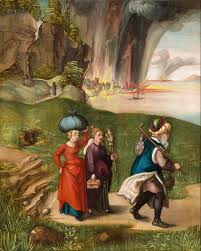
\includegraphics[height=6cm]{img/candc/DurerLotandDaughters.jpg}
	\caption{Albrecht Durer - Lot and his Daughters (c.1496/1499}
	\label{fig:DurerLotAndDaughters}
\end{figure}
\end{frame}
\begin{center}\line(1,0){250}\end{center}




\begin{frame}
\frametitle{Tell a Story or Capture a Moment}
\begin{figure}
	\centering
		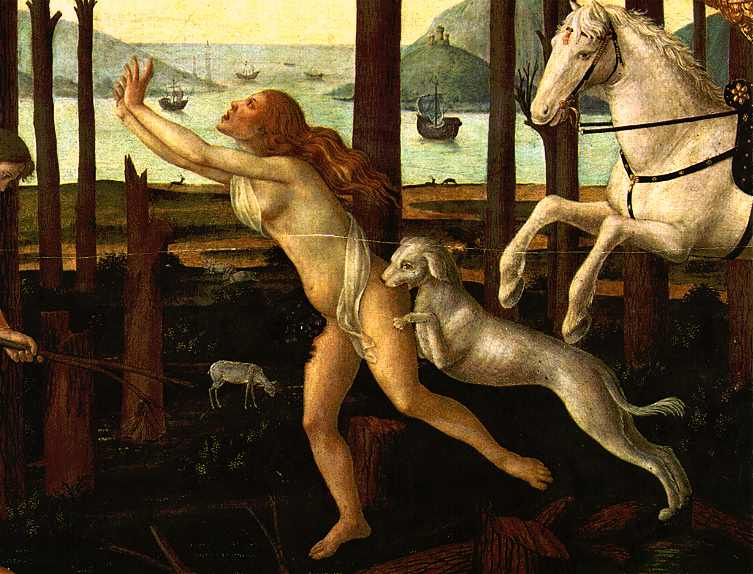
\includegraphics[height=6cm]{img/candc/nastag12.jpg}
	\caption{Sandro Botticelli - The Story of Nastagio degli Onesti (c.1483)}
	\label{fig:BotticelliNastagio}
\end{figure}
\end{frame}
\begin{center}\line(1,0){250}\end{center}



\begin{frame}
\frametitle{Use Light to direct attention}
\begin{figure}
	\centering
		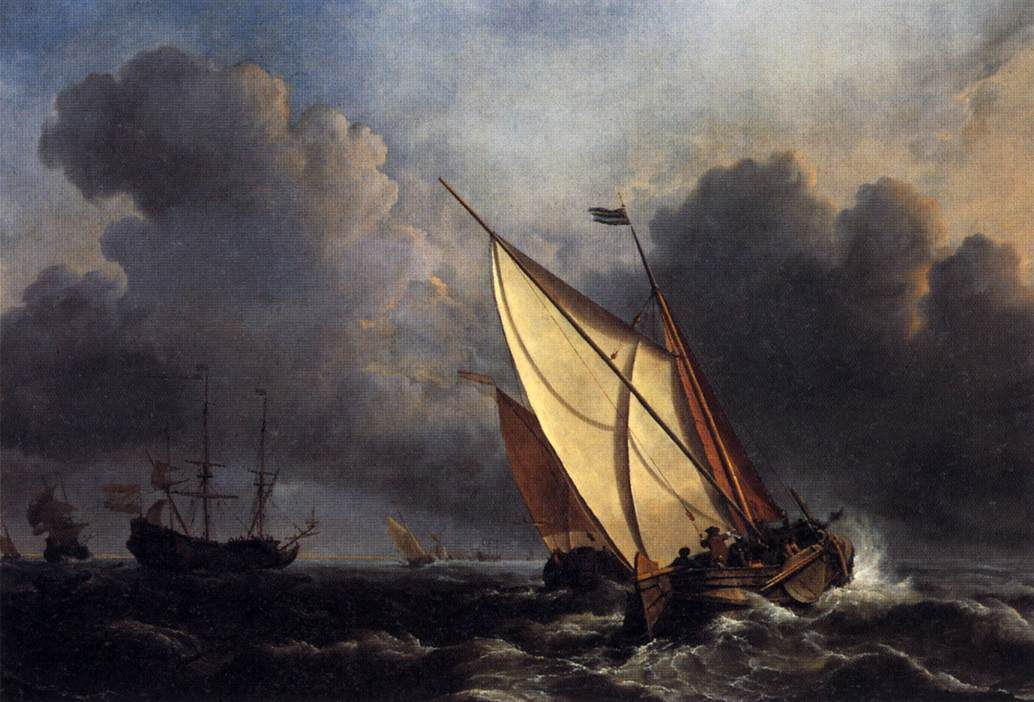
\includegraphics[height=6cm]{img/candc/TurnerFishingBoatsStorm.jpg}
	\caption{William Turner - Dutch Fishing Boats in a Storm (1801)}
	\label{fig:WilliamTurnerFishingBoat}
\end{figure}
\end{frame}
\begin{center}\line(1,0){250}\end{center}



\begin{frame}
\frametitle{Use Light to direct attention}
\begin{figure}
	\centering
		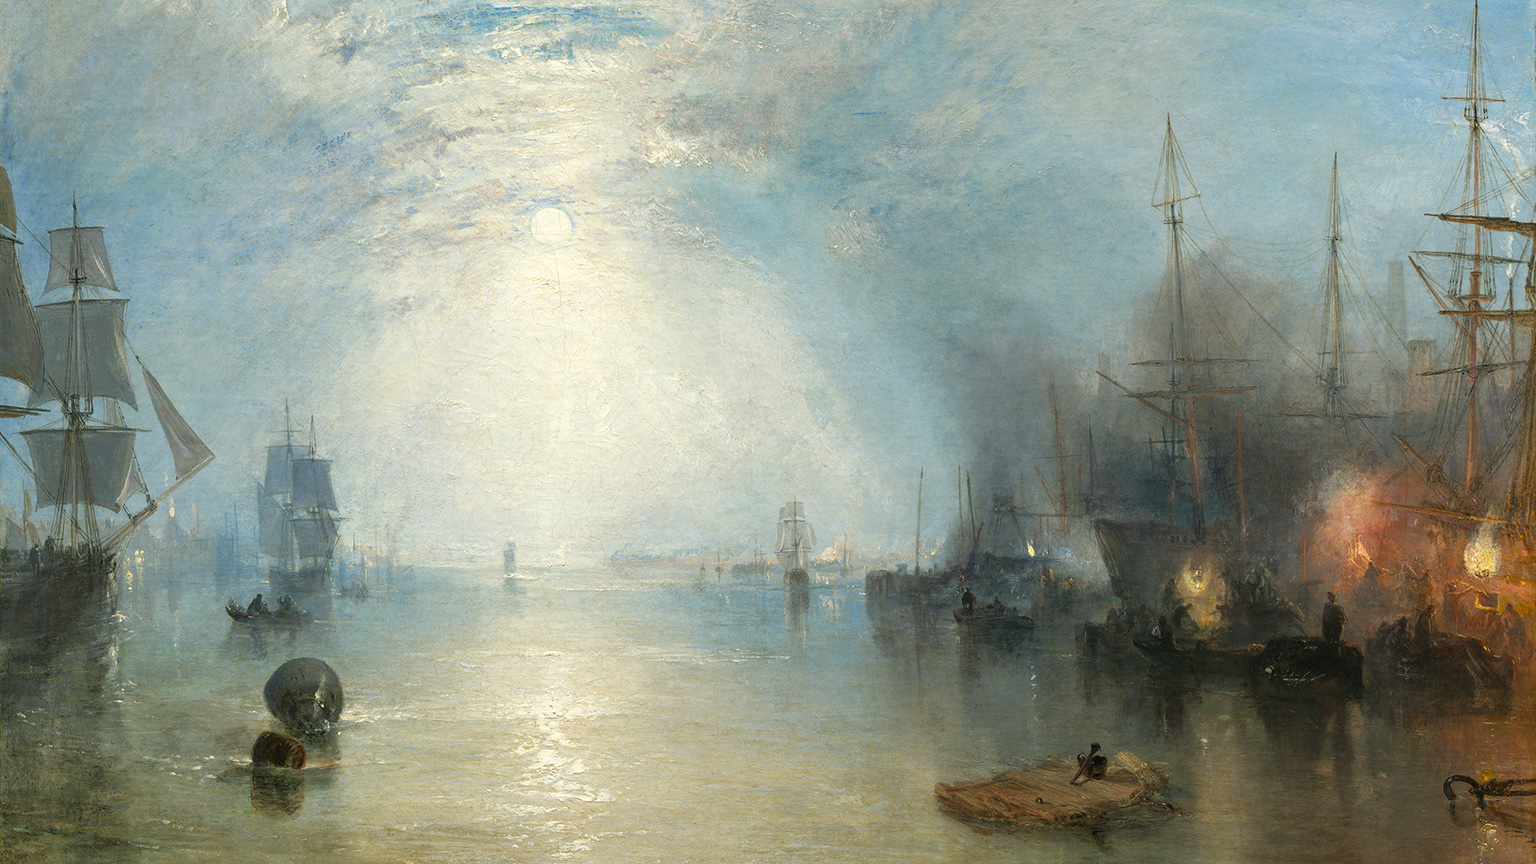
\includegraphics[height=6cm]{img/candc/TurnerCoal-by-Moonlight.jpg}
	\caption{William Turner - Keelmen Heaving in Coals by Moonlight (1835)}
	\label{fig:williamTurnerKeelmen}
\end{figure}
\end{frame}
\begin{center}\line(1,0){250}\end{center}




\begin{frame}
\frametitle{Use Light to direct attention}
\begin{figure}
	\centering
		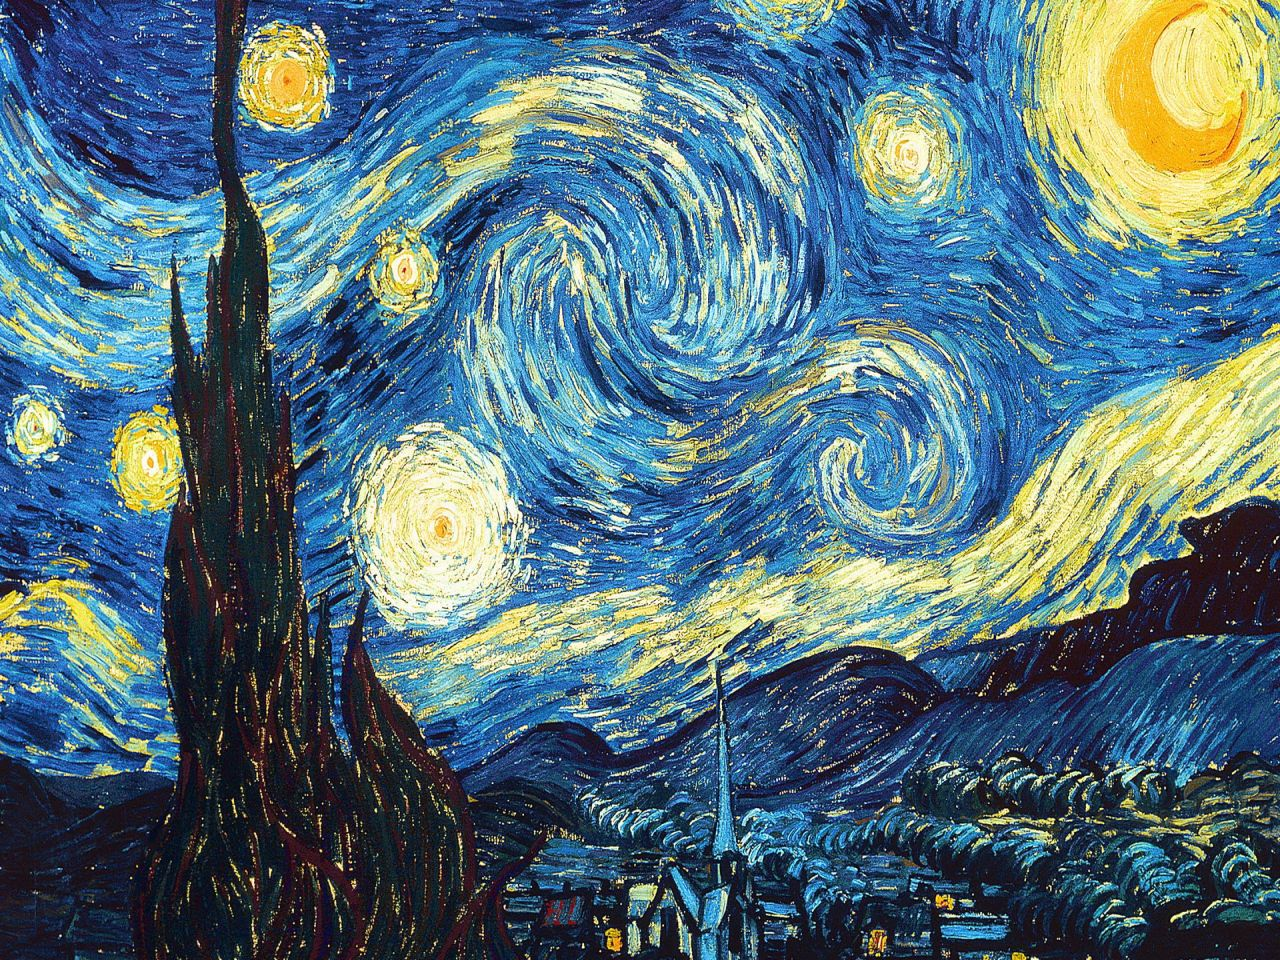
\includegraphics[height=6cm]{img/candc/starry-night-VanGogh.jpg}
	\caption{Vincent van Gogh - The Starry Night (1889)}
	\label{fig:starrynight}
\end{figure}
\end{frame}
\begin{center}\line(1,0){250}\end{center}




\begin{frame}
\frametitle{Framing}
\begin{figure}
	\centering
	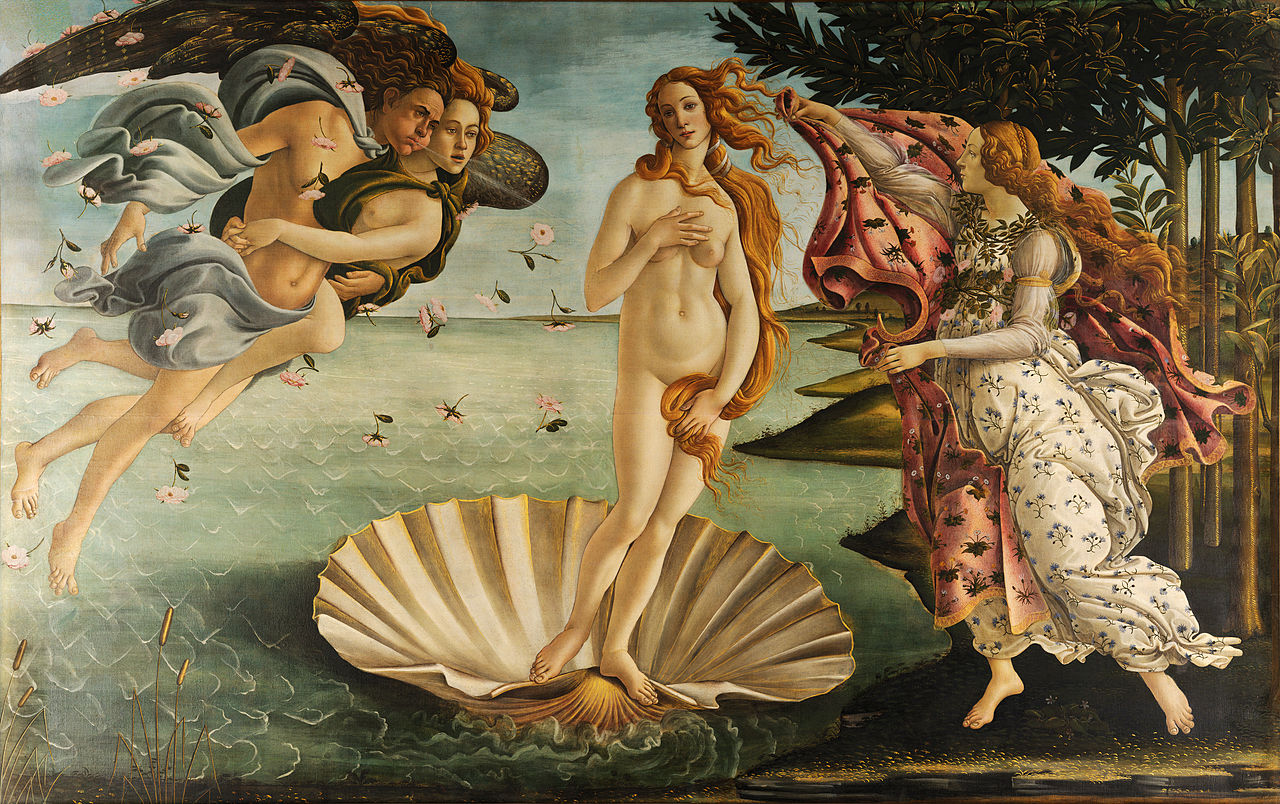
\includegraphics[width=0.7\linewidth]{img/CandC/1280px-Sandro_Botticelli_-_La_nascita_di_Venere_-_Google_Art_Project_-_edited}
	\caption[Sandro Botticelli - The Birth of Venus, c.1485]{Sandro Botticelli - The Birth of Venus, c.1485}
	\label{fig:sandrobotticelliVenus}
\end{figure}
\end{frame}
\begin{center}\line(1,0){250}\end{center}


\begin{frame}
\frametitle{Framing}
\begin{figure}
	\centering
	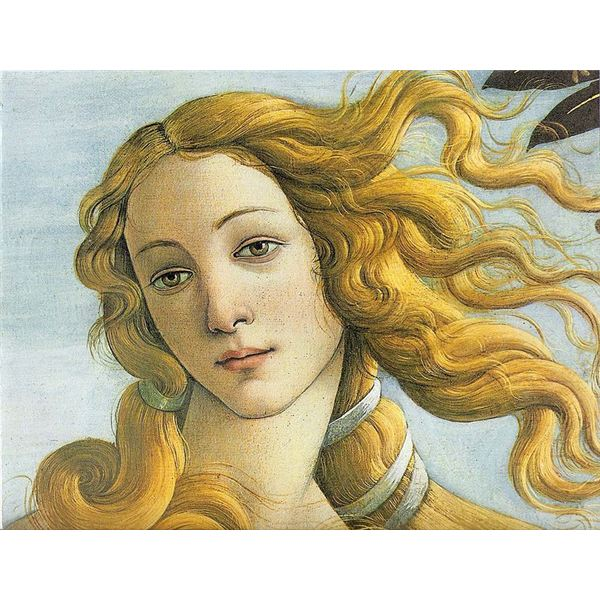
\includegraphics[width=0.7\linewidth]{img/CandC/BirthofVenusCrop.jpg}
	\caption[Sandro Botticelli - The Birth of Venus, c.1485]{Sandro Botticelli - The Birth of Venus, c.1485}
	\label{fig:sandrobotticelliVenus}
\end{figure}
\end{frame}
\begin{center}\line(1,0){250}\end{center}



\begin{frame}
\frametitle{Framing}
\begin{figure}
	\centering
	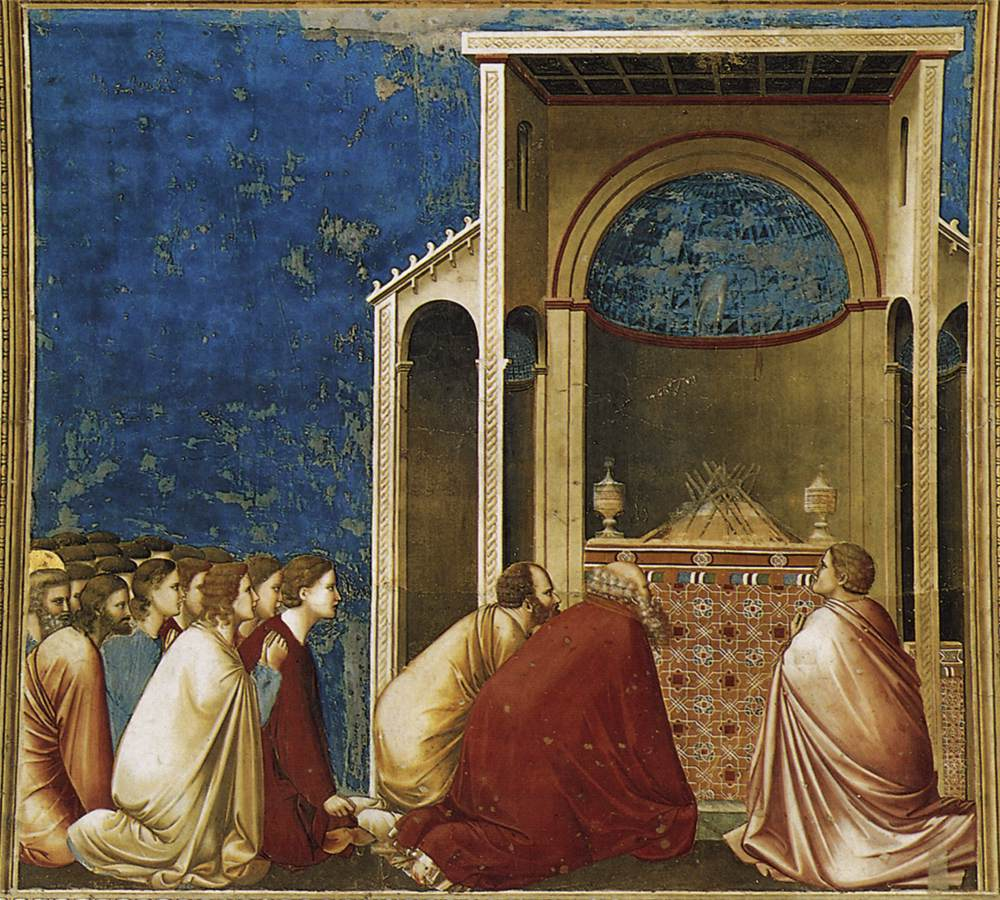
\includegraphics[width=0.7\linewidth]{img/CandC/the-suitors-praying}
	\caption{Giotto - The Suitors Praying (1306)}
	\label{fig:the-suitors-praying}
\end{figure}
\end{frame}
\begin{center}\line(1,0){250}\end{center}



\begin{frame}
\frametitle{Framing}
\begin{figure}
	\centering
	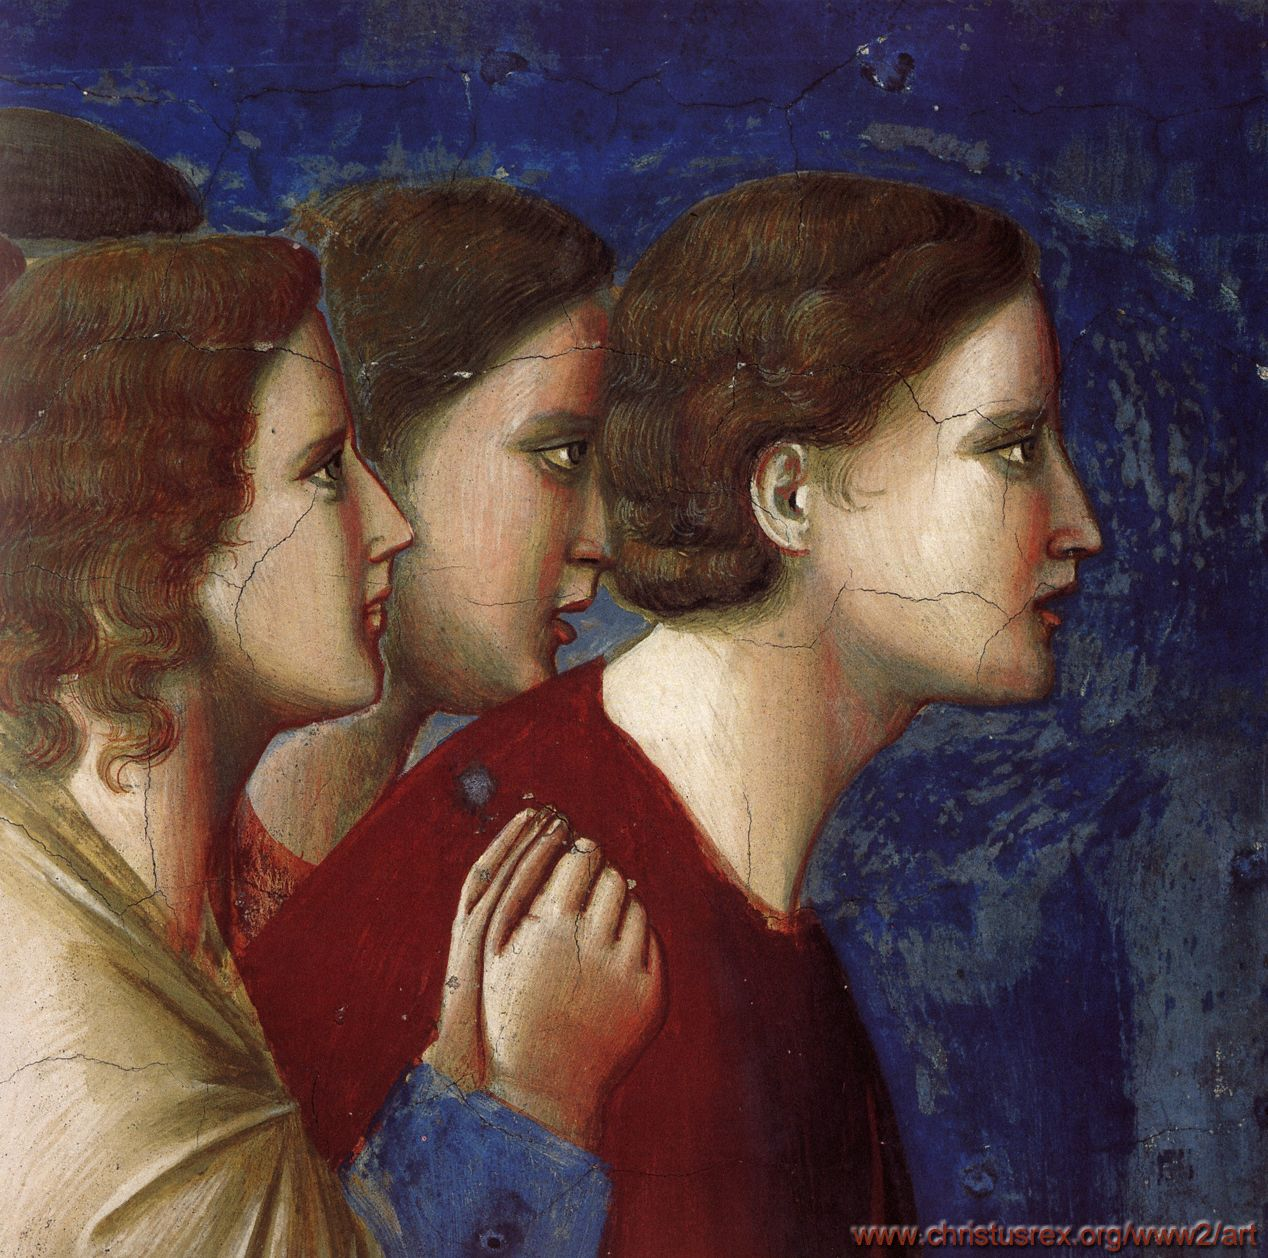
\includegraphics[width=0.7\linewidth]{img/CandC/giotto3a}
	\caption{Giotto - The Suitors Praying (1306)}
	\label{fig:giotto3a}
\end{figure}
\end{frame}
\begin{center}\line(1,0){250}\end{center}R





\begin{frame}
\frametitle{Suggest a Story}
\begin{figure}
	\centering
		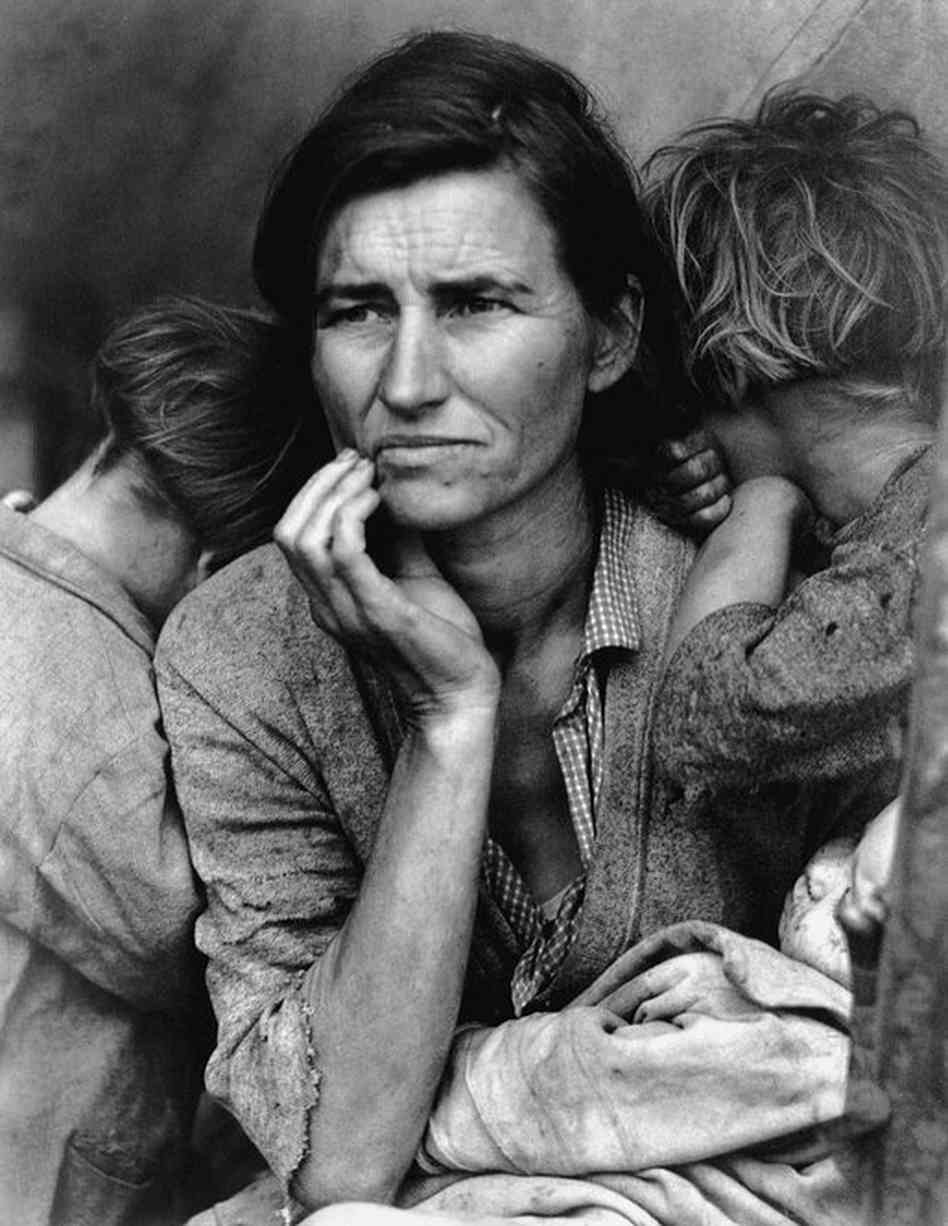
\includegraphics[height=6cm]{img/candc/DorethaLange.jpg}
	\caption{Dorothea Lange - Migrant Mother (California, 1936)}
	\label{fig:DorotheaLangeMigrantMother}
\end{figure}
\end{frame}
\begin{center}\line(1,0){250}\end{center}


\begin{frame}
\frametitle{Suggest a Story}
\begin{figure}
	\centering
		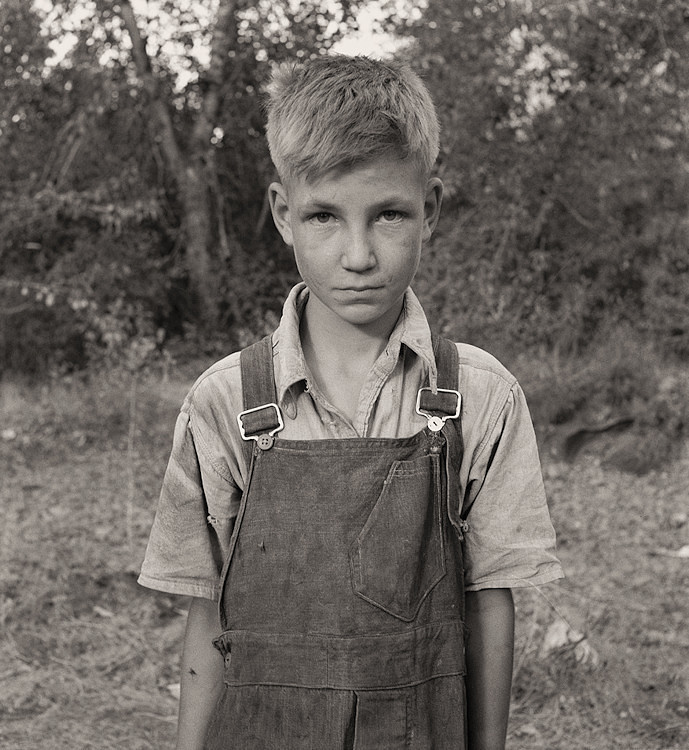
\includegraphics[height=6cm]{img/candc/DorethaLange2.jpg}
	\caption{Dorothea Lange}
	\label{fig:DorotheaLange2}
\end{figure}
\end{frame}
\begin{center}\line(1,0){250}\end{center}



\begin{frame}
\frametitle{Suggest a Story}
\begin{figure}
	\centering
		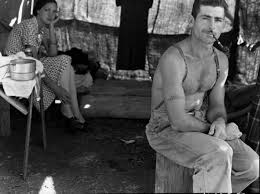
\includegraphics[height=6cm]{img/candc/DorethaLange3.jpg}
	\caption{Dorothea Lange}
	\label{fig:DorotheaLange3}
\end{figure}
\end{frame}
\begin{center}\line(1,0){250}\end{center}





\begin{frame}
\frametitle{Who Lives Here?}
\begin{figure}
	\centering
		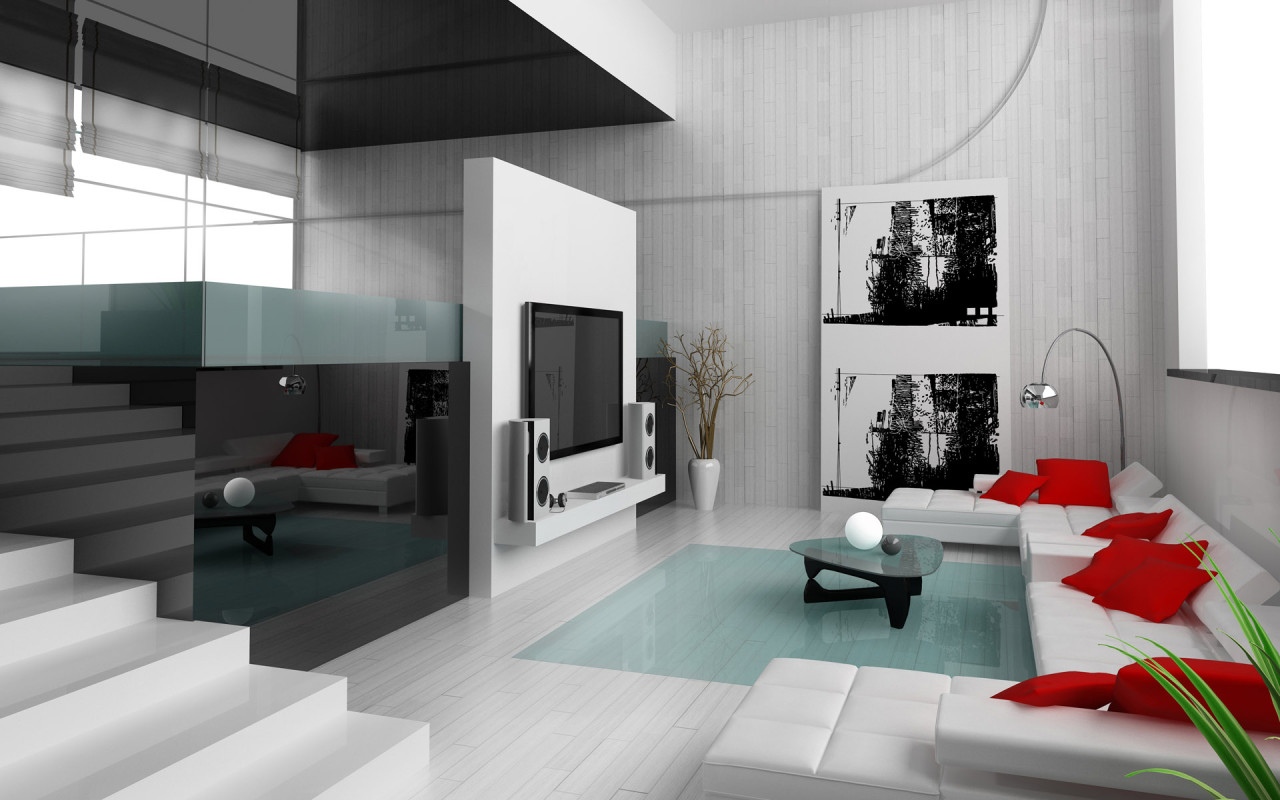
\includegraphics[height=6cm]{img/A.jpg}
	\caption{TEST Image}
	\label{fig:lightingtypes}
\end{figure}
\end{frame}
\begin{center}\line(1,0){250}\end{center}



\begin{frame}
\frametitle{Who Lives Here?}
\begin{figure}
	\centering
		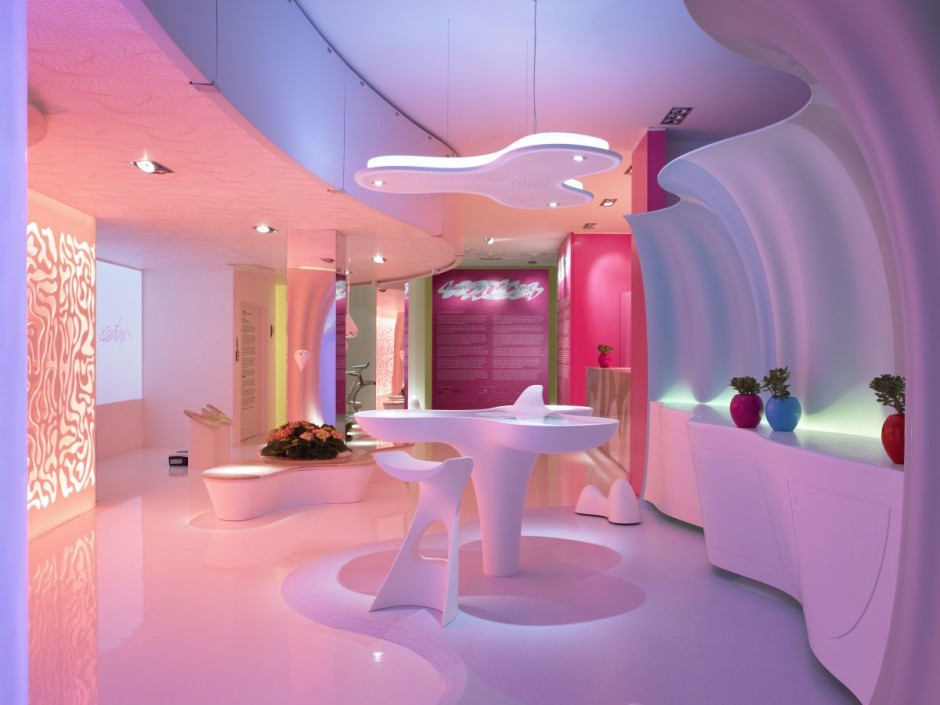
\includegraphics[height=6cm]{img/A1.jpg}
	\caption{TEST Image}
	\label{fig:lightingtypes}
\end{figure}
\end{frame}
\begin{center}\line(1,0){250}\end{center}



\begin{frame}
\frametitle{Who Lives Here?}
\begin{figure}
	\centering
		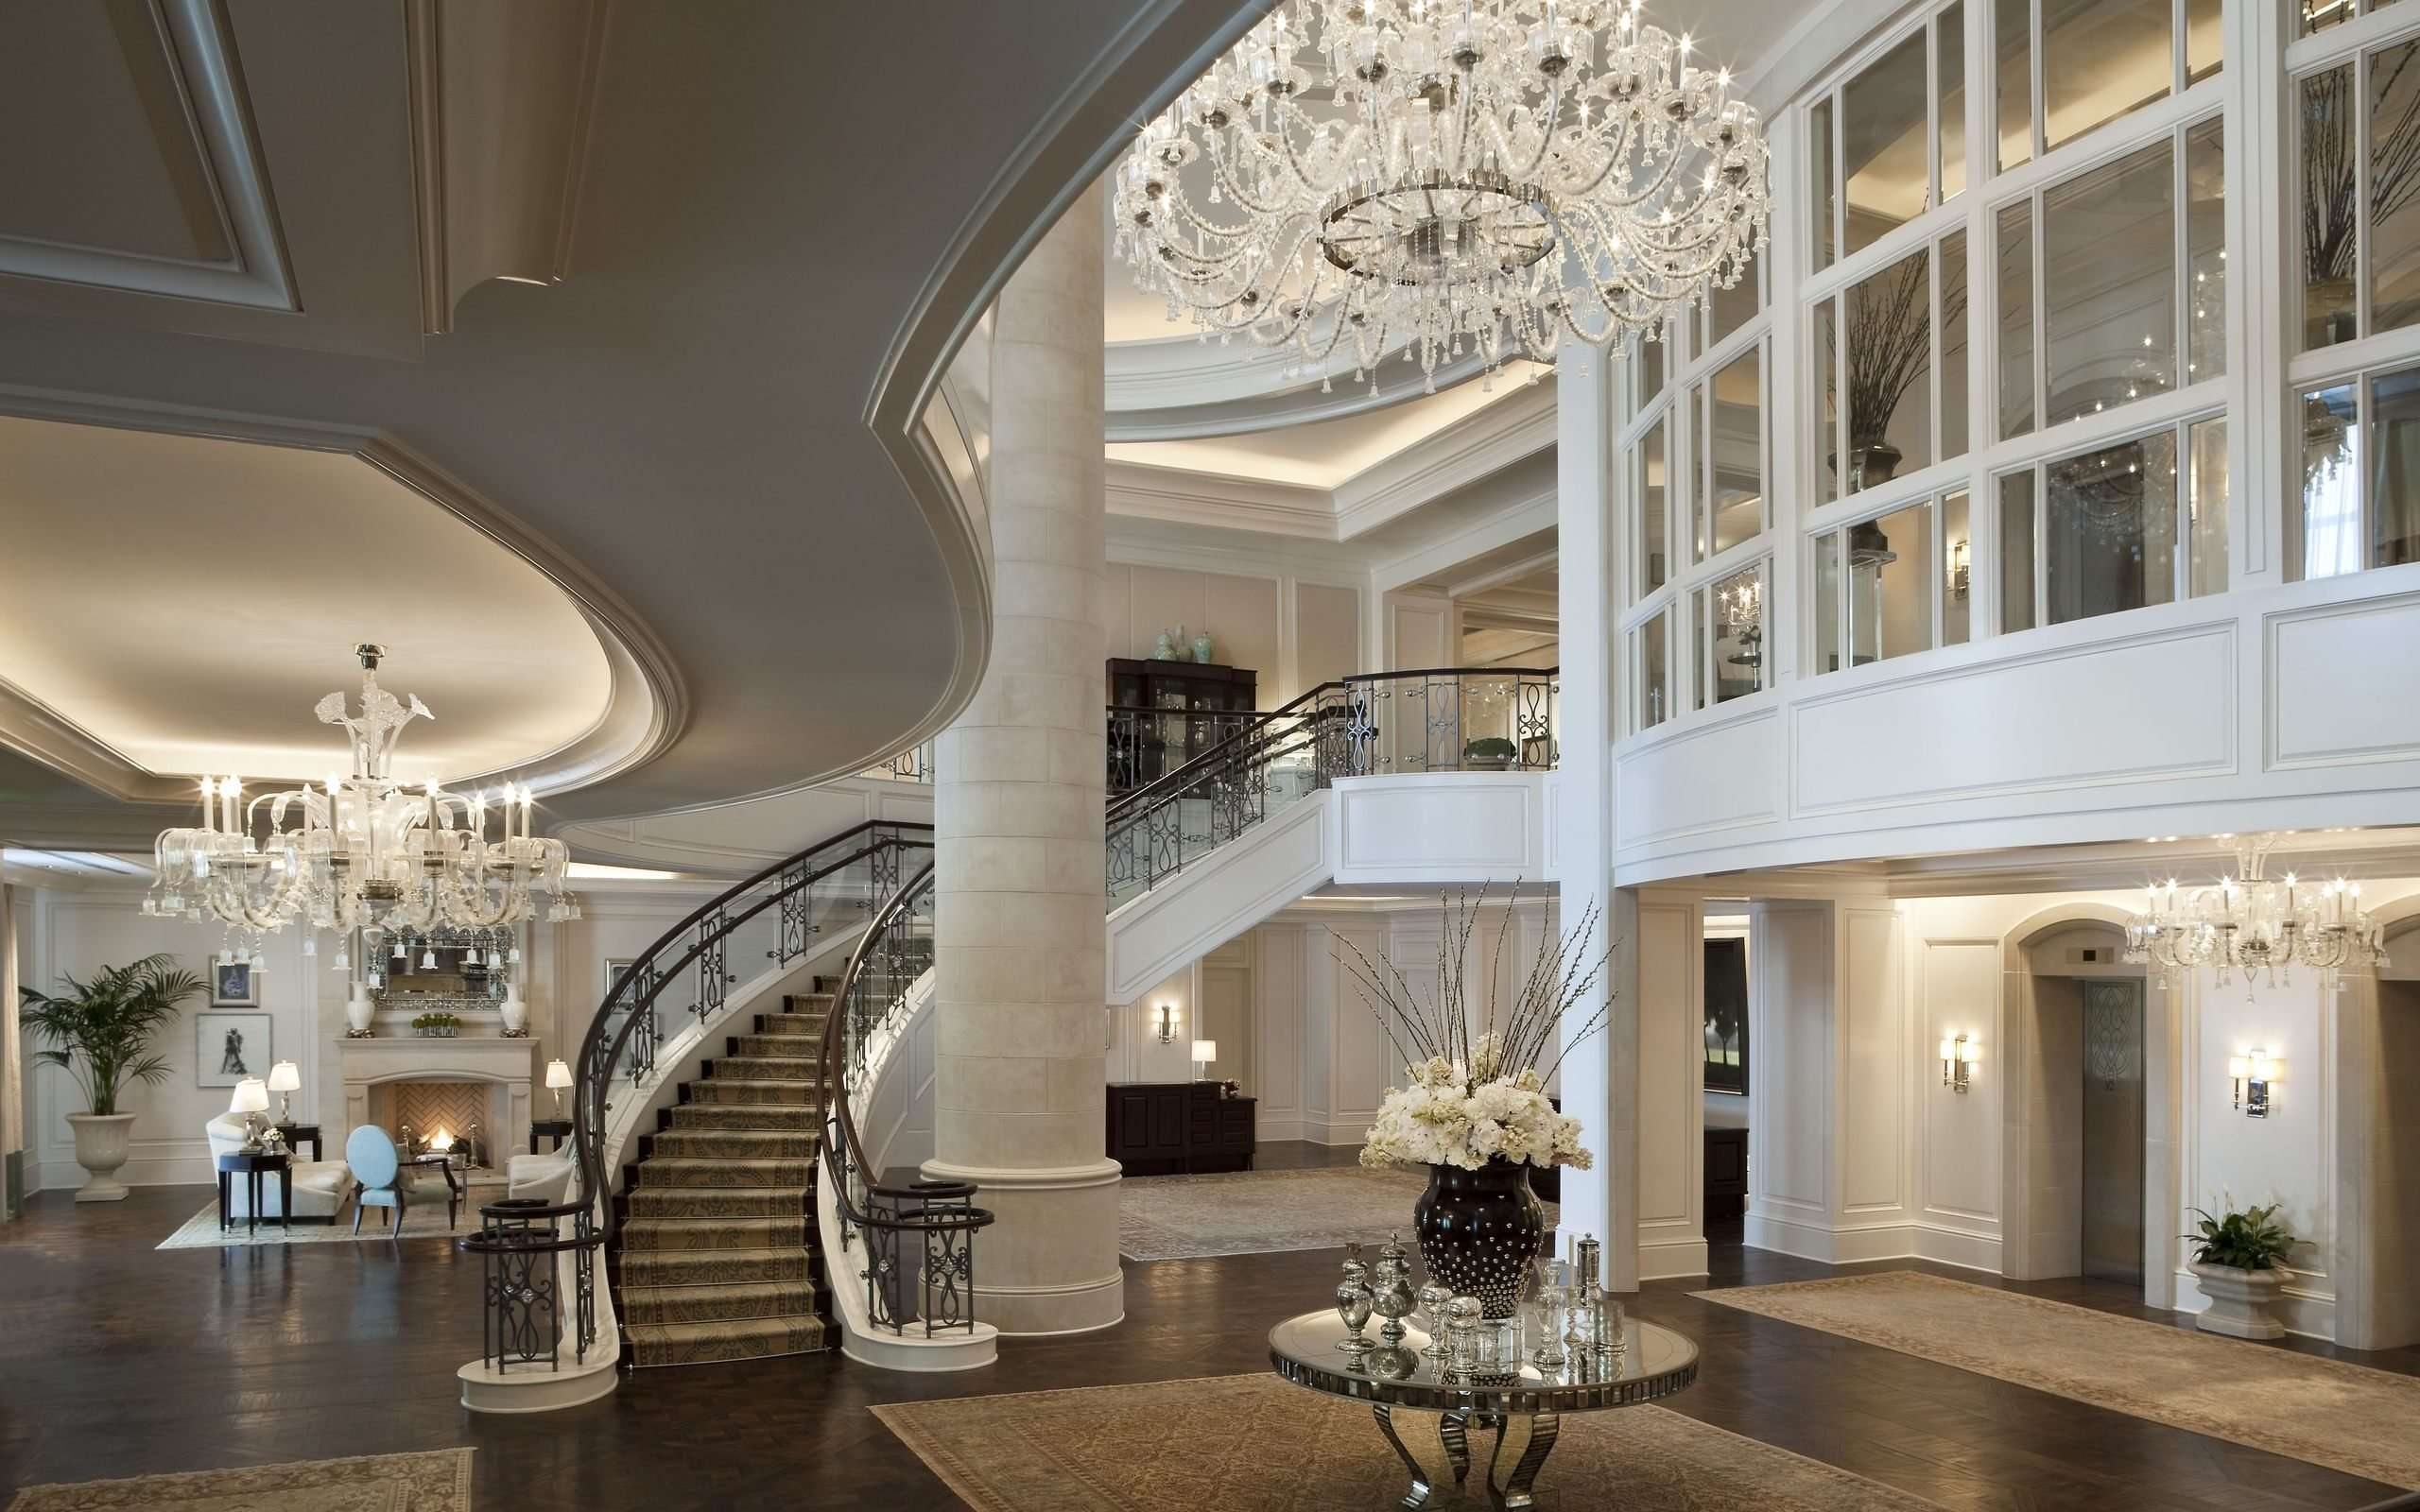
\includegraphics[height=6cm]{img/B.jpg}
	\caption{TEST Image}
	\label{fig:lightingtypes}
\end{figure}
\end{frame}
\begin{center}\line(1,0){250}\end{center}



\begin{frame}
\frametitle{Who Lives Here?}
\begin{figure}
	\centering
		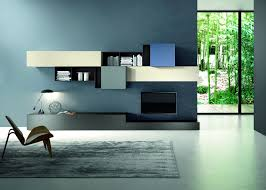
\includegraphics[height=6cm]{img/C.jpg}
	\caption{TEST Image}
	\label{fig:lightingtypes}
\end{figure}
\end{frame}
\begin{center}\line(1,0){250}\end{center}



\begin{frame}
\frametitle{Who Lives Here?}
\begin{figure}
	\centering
		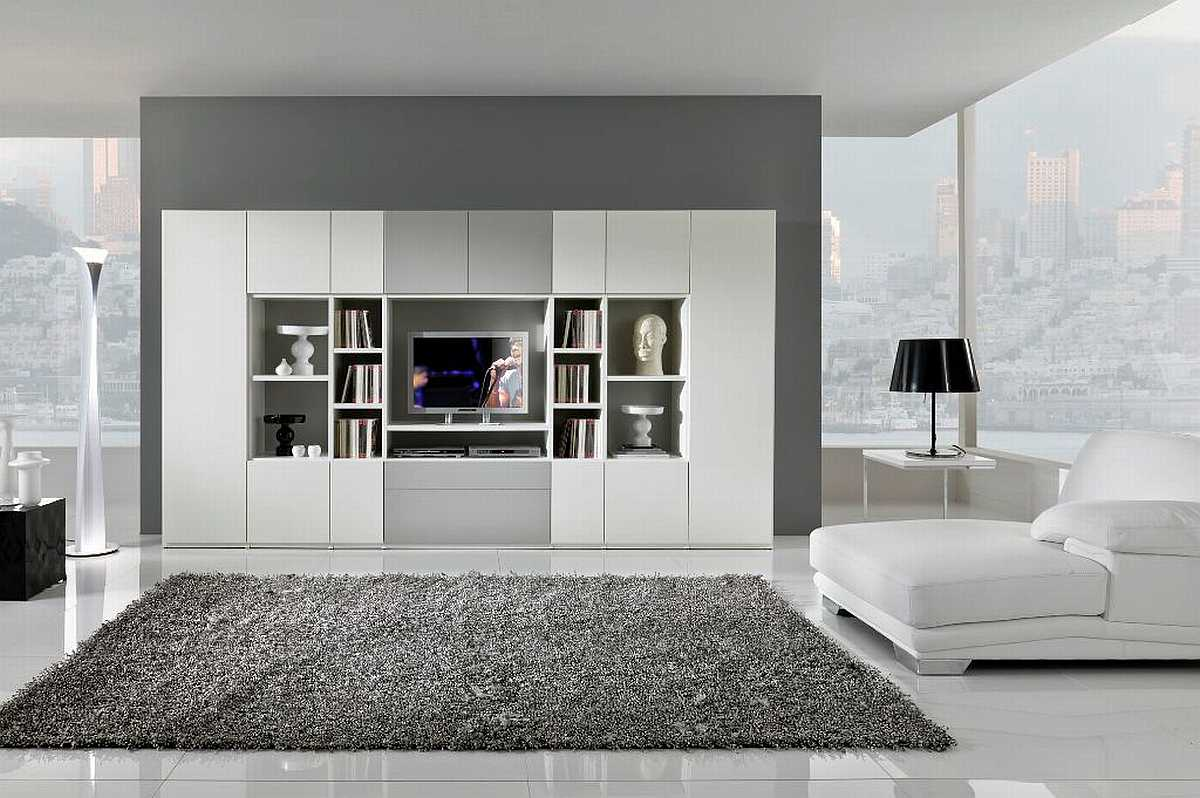
\includegraphics[height=6cm]{img/D.jpg}
	\caption{TEST Image}
	\label{fig:lightingtypes}
\end{figure}
\end{frame}
\begin{center}\line(1,0){250}\end{center}



\begin{frame}
\frametitle{Who Lives Here?}
\begin{figure}
	\centering
		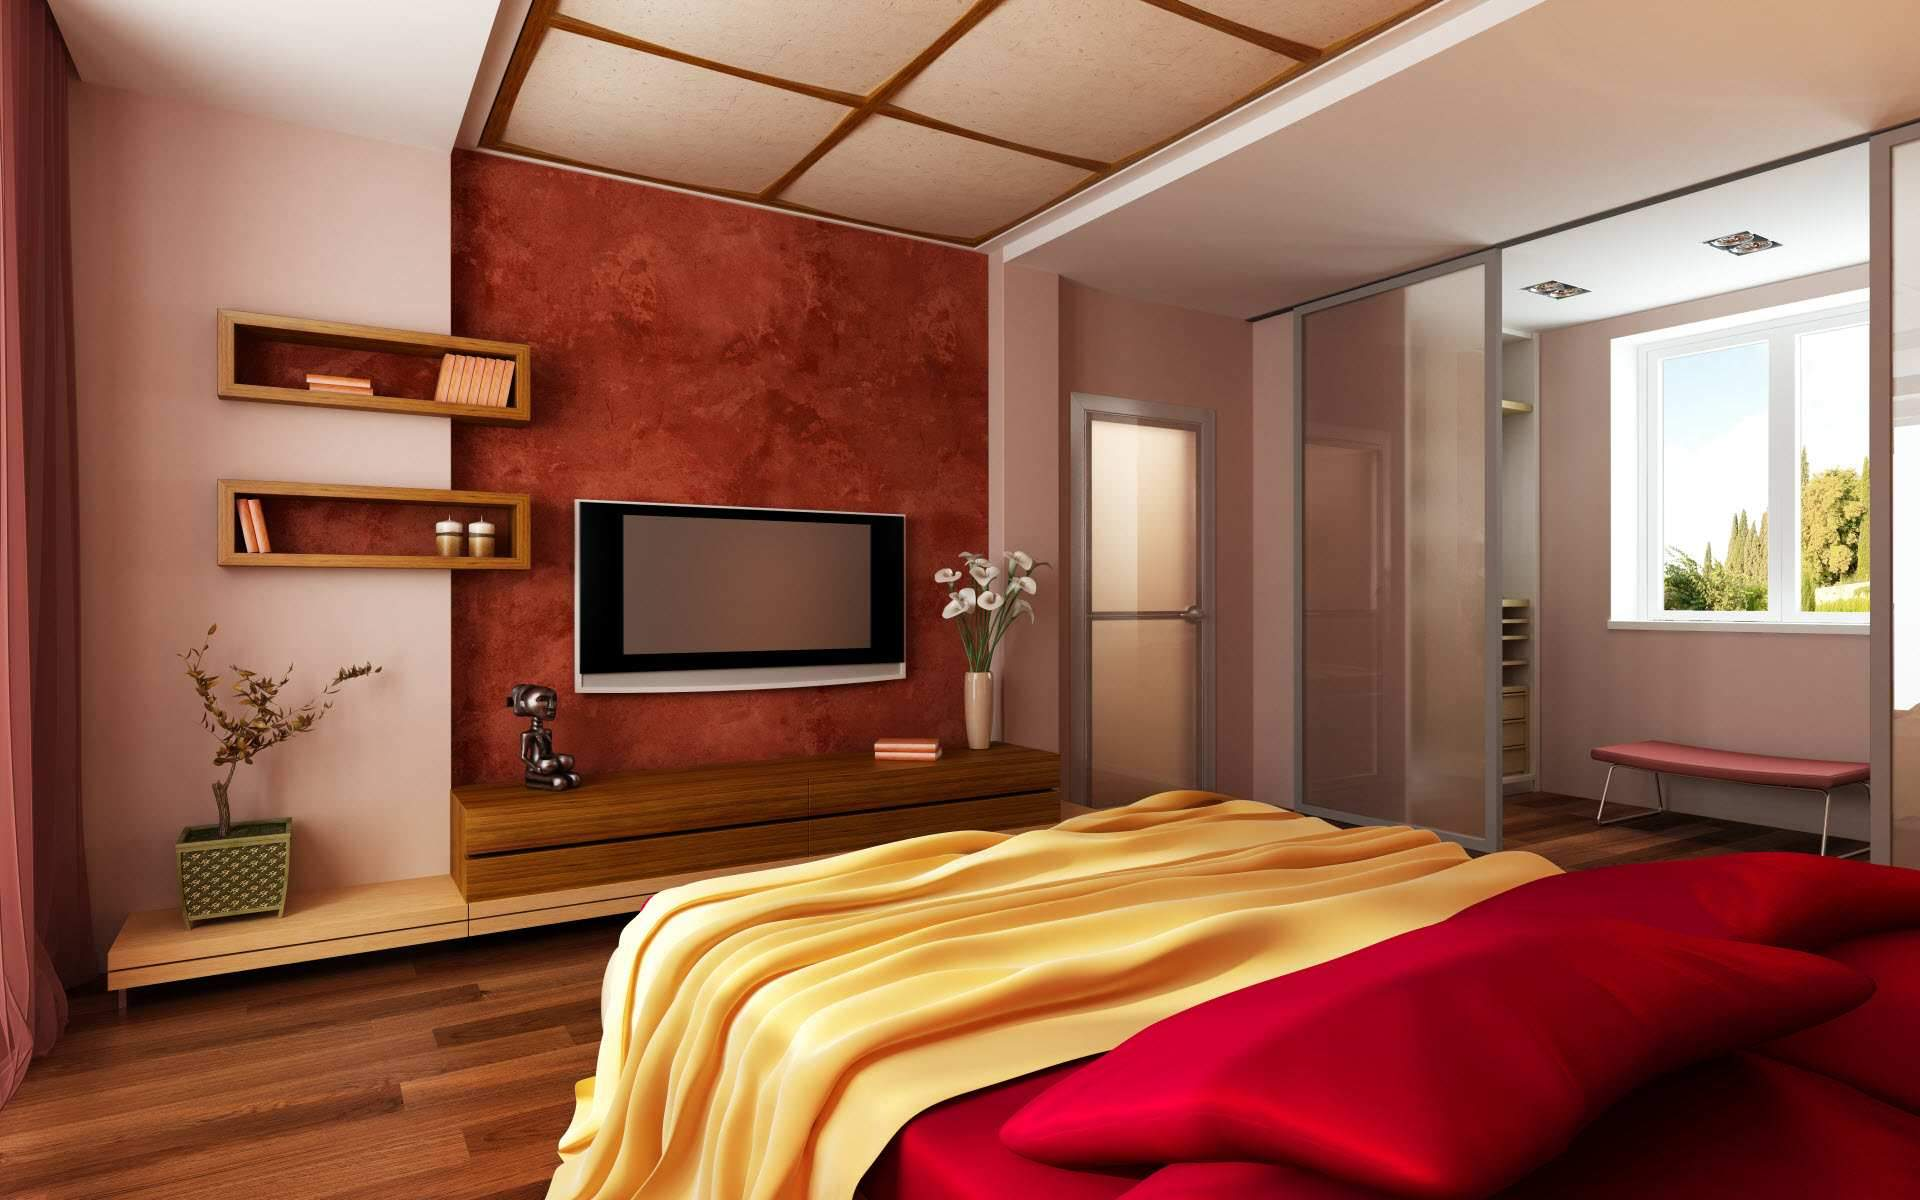
\includegraphics[height=6cm]{img/E.jpg}
	\caption{TEST Image}
	\label{fig:lightingtypes}
\end{figure}
\end{frame}
\begin{center}\line(1,0){250}\end{center}




\begin{frame}
\frametitle{Who Lives Here?}
\begin{figure}
	\centering
		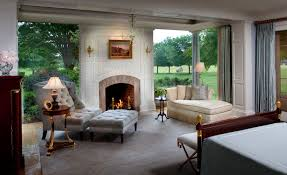
\includegraphics[height=6cm]{img/F.jpg}
	\caption{TEST Image}
	\label{fig:lightingtypes}
\end{figure}
\end{frame}
\begin{center}\line(1,0){250}\end{center}




\begin{frame}
\frametitle{Who Lives Here?}
\begin{figure}
	\centering
		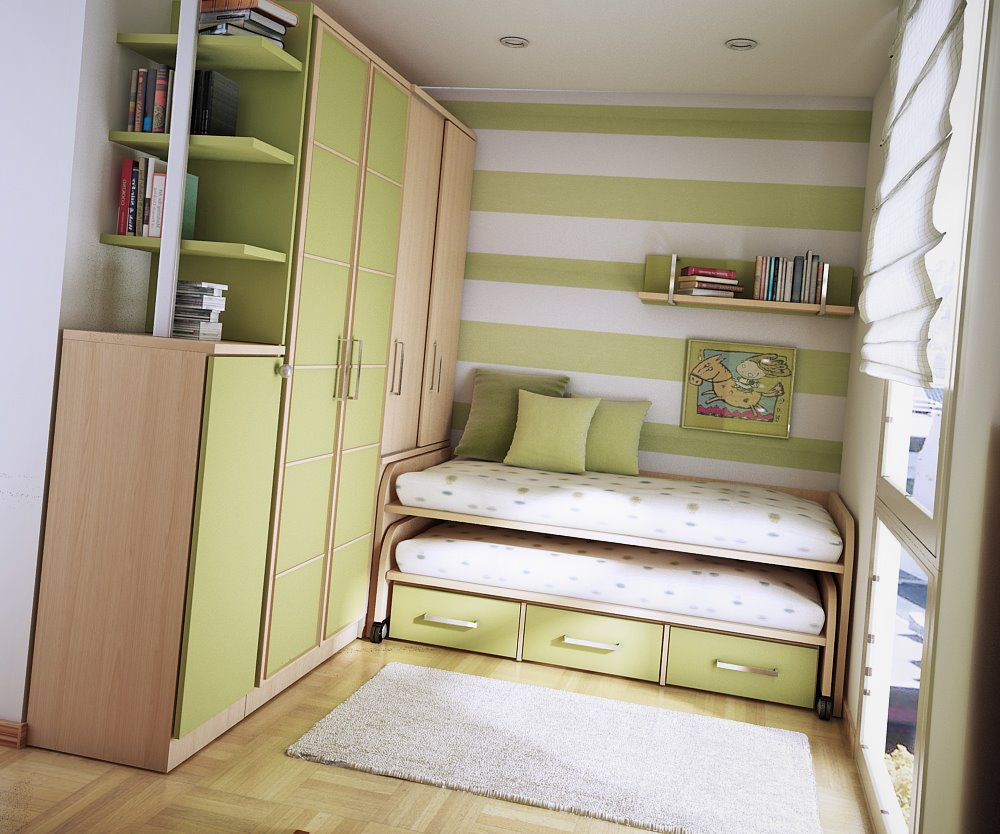
\includegraphics[height=6cm]{img/G.jpg}
	\caption{TEST Image}
	\label{fig:lightingtypes}
\end{figure}
\end{frame}
\begin{center}\line(1,0){250}\end{center}




\begin{frame}
\frametitle{Who Lives Here?}
\begin{figure}
	\centering
		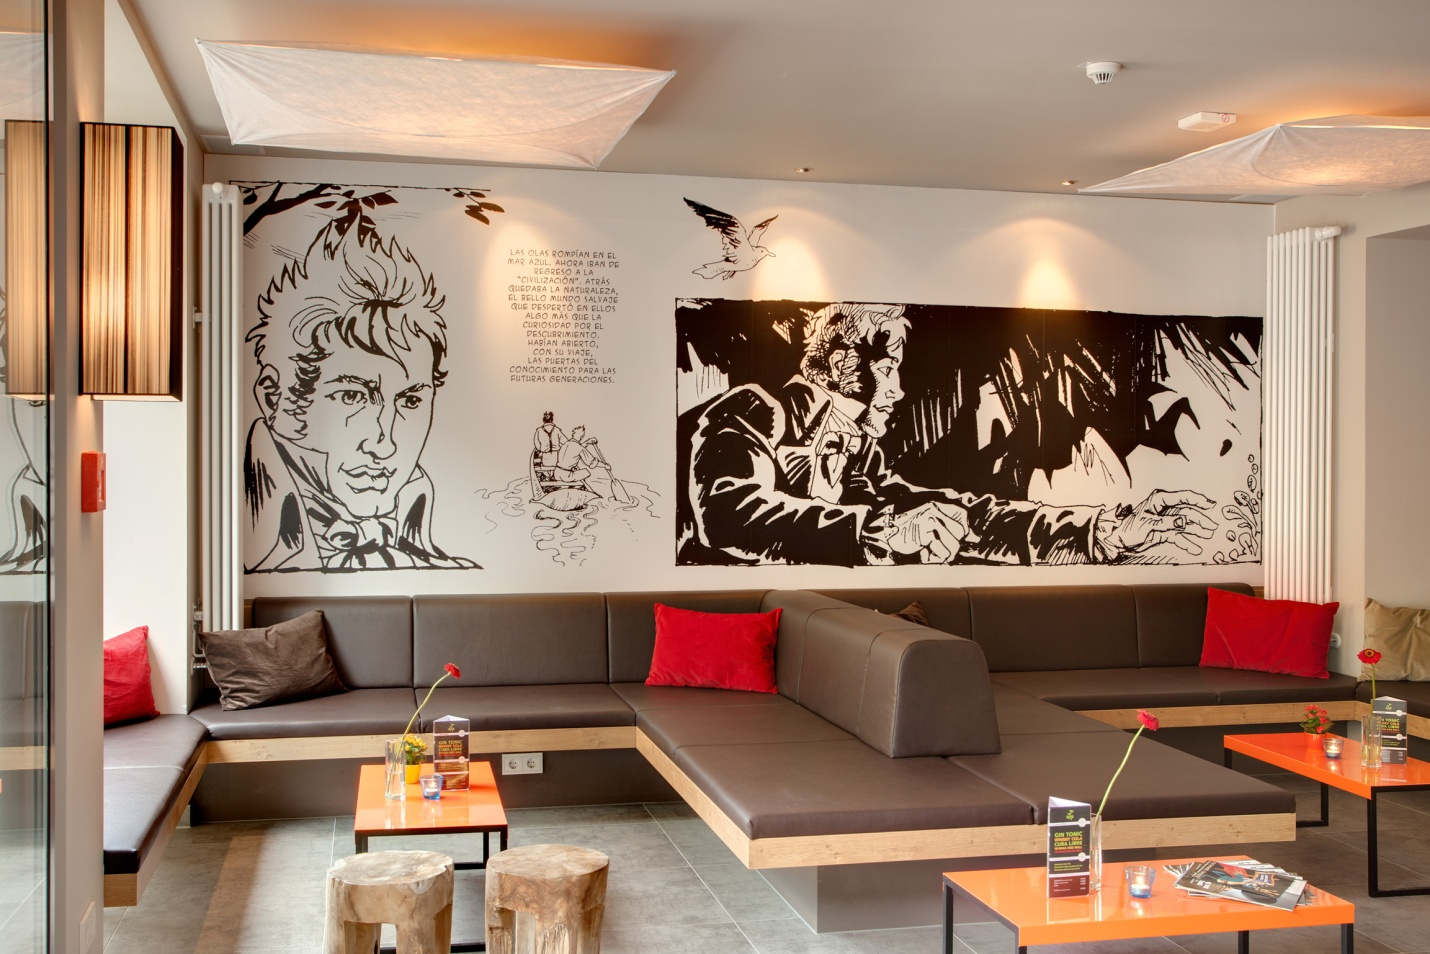
\includegraphics[height=6cm]{img/H.jpg}
	\caption{TEST Image}
	\label{fig:lightingtypes}
\end{figure}
\end{frame}
\begin{center}\line(1,0){250}\end{center}




\begin{frame}
\frametitle{Who Lives Here?}
\begin{figure}
	\centering
		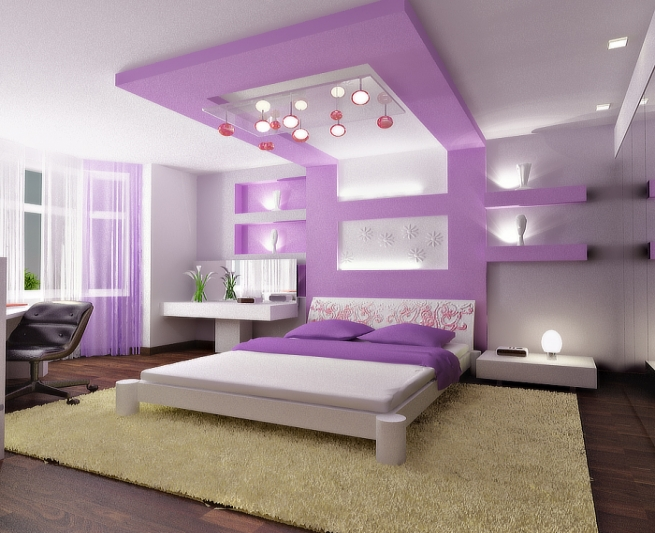
\includegraphics[height=6cm]{img/H.png}
	\caption{TEST Image}
	\label{fig:lightingtypes}
\end{figure}
\end{frame}
\begin{center}\line(1,0){250}\end{center}



\begin{frame}
\frametitle{Who Lives Here?}
\begin{figure}
	\centering
		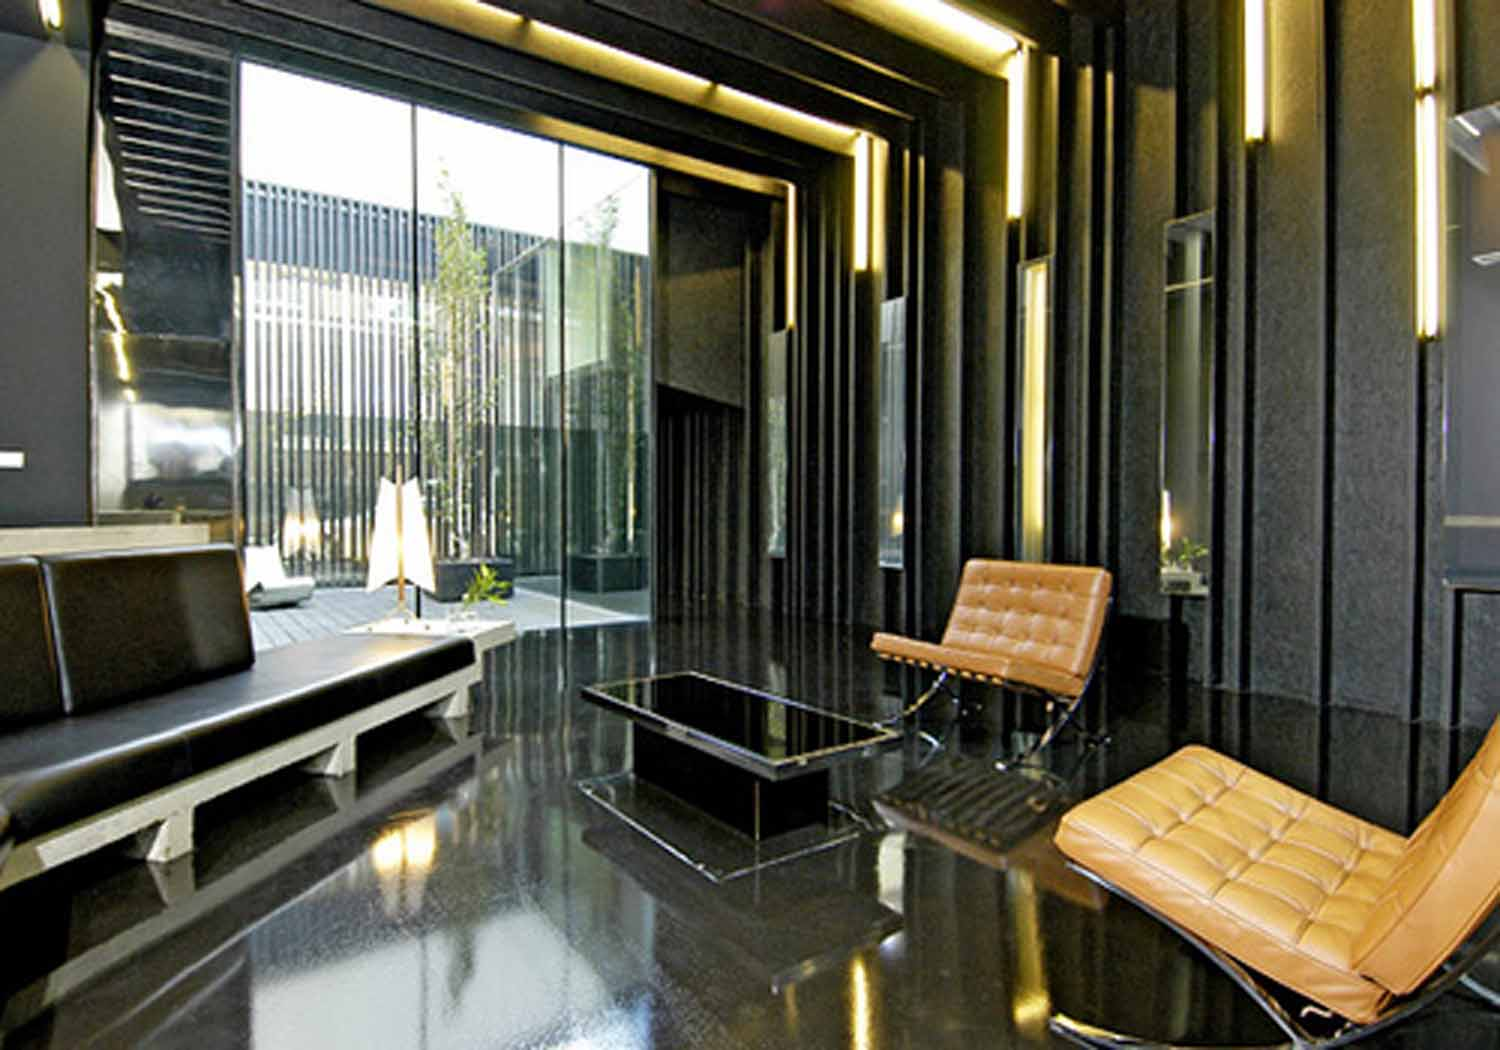
\includegraphics[height=6cm]{img/J.jpg}
	\caption{TEST Image}
	\label{fig:lightingtypes}
\end{figure}
\end{frame}
\begin{center}\line(1,0){250}\end{center}



\begin{frame}
\frametitle{Who Lives Here?}
\begin{figure}
	\centering
		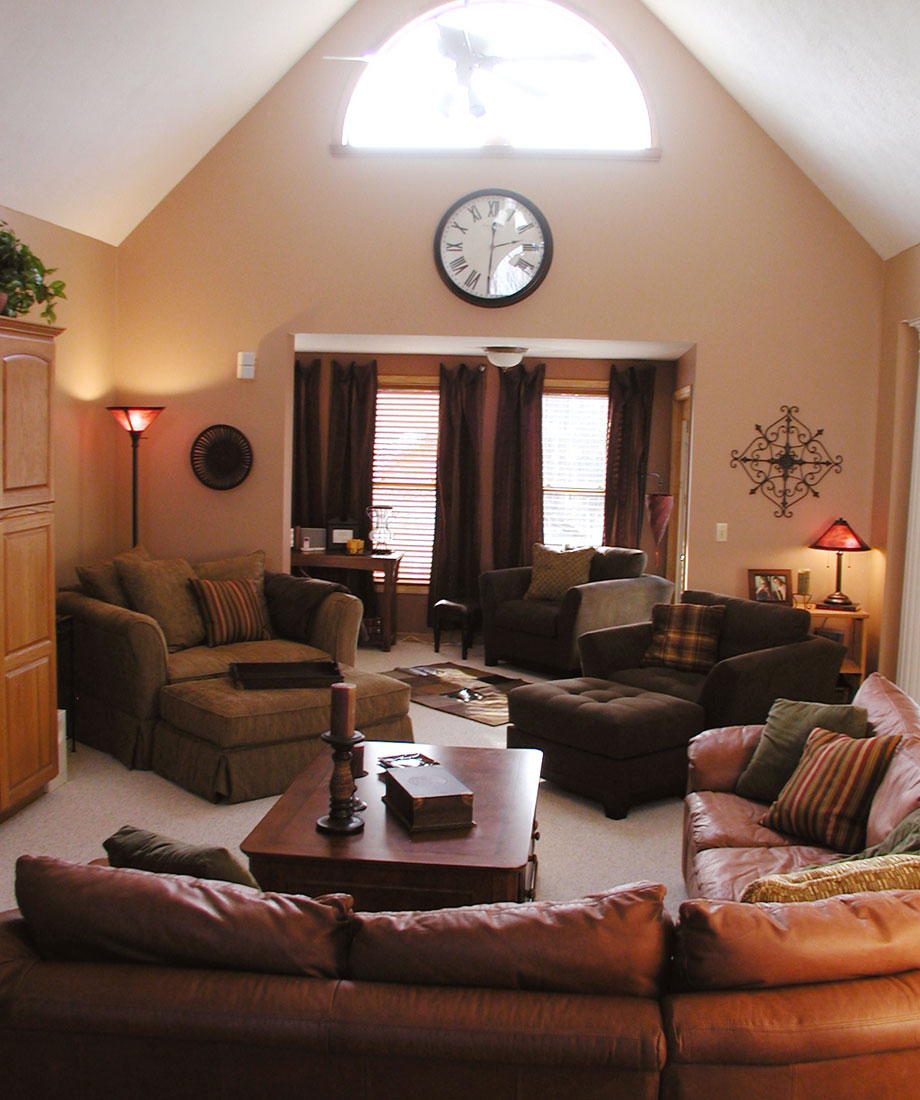
\includegraphics[height=6cm]{img/K.jpg}
	\caption{TEST Image}
	\label{fig:lightingtypes}
\end{figure}
\end{frame}
\begin{center}\line(1,0){250}\end{center}



\begin{frame}
\frametitle{User Story}
\begin{itemize}
	\item A user story is a simple way of describing how we expect a user to interact with the space we have created.
	\item It is a common design technique; used in early stage design to create a better understanding of the design functionality requirements
	\item In our case we are going to use this technique to develop images that will sit well with our clients
\end{itemize}
\end{frame}
\begin{center}\line(1,0){250}\end{center}



\begin{frame}
\frametitle{User Story \hfill\hfill Typical Components}
\begin{itemize}
	\item Demographic Profile; Age, Sex, etc.
	\item Space Usage; how will the user interact with this space; what will they do, when, how often, etc.
	\item By understanding these elements, we can create images that feed into the users expectations.
	\item We can give them names, family, or anything else that will allow us to develop a better understanding of their needs.
\end{itemize}
\end{frame}
\begin{center}\line(1,0){250}\end{center}



\begin{frame}
\frametitle{User Story \hfill\hfill Typical Components}
\begin{itemize}
	\item Demographic Profile; Age, Sex, etc.
	\item Space Usage; how will the user interact with this space; what will they do, when, how often, etc.
	\item By understanding these elements, we can create images that feed into the users expectations.
	\item We can give them names, family, or anything else that will allow us to develop a better understanding of their needs.
\end{itemize}
\end{frame}
\begin{center}\line(1,0){250}\end{center}





\begin{frame}
\frametitle{User Story \hfill\hfill Example}
\begin{itemize}
	\item Robert and Georgina have been married for 3 years.  They intend to have children, but not for a few years.  They have good jobs and have a reasonable disposable income.  They like living in the city but prefer the great outdoors.  They recently inherited some land, and would like to build a weekend home.  They are adamant that their new home must blend in with the landscape, and be capable of expansion when children arrive.
\end{itemize}
\end{frame}
\begin{center}\line(1,0){250}\end{center}


\begin{frame}
\frametitle{User Story Result}
\begin{figure}
	\centering
		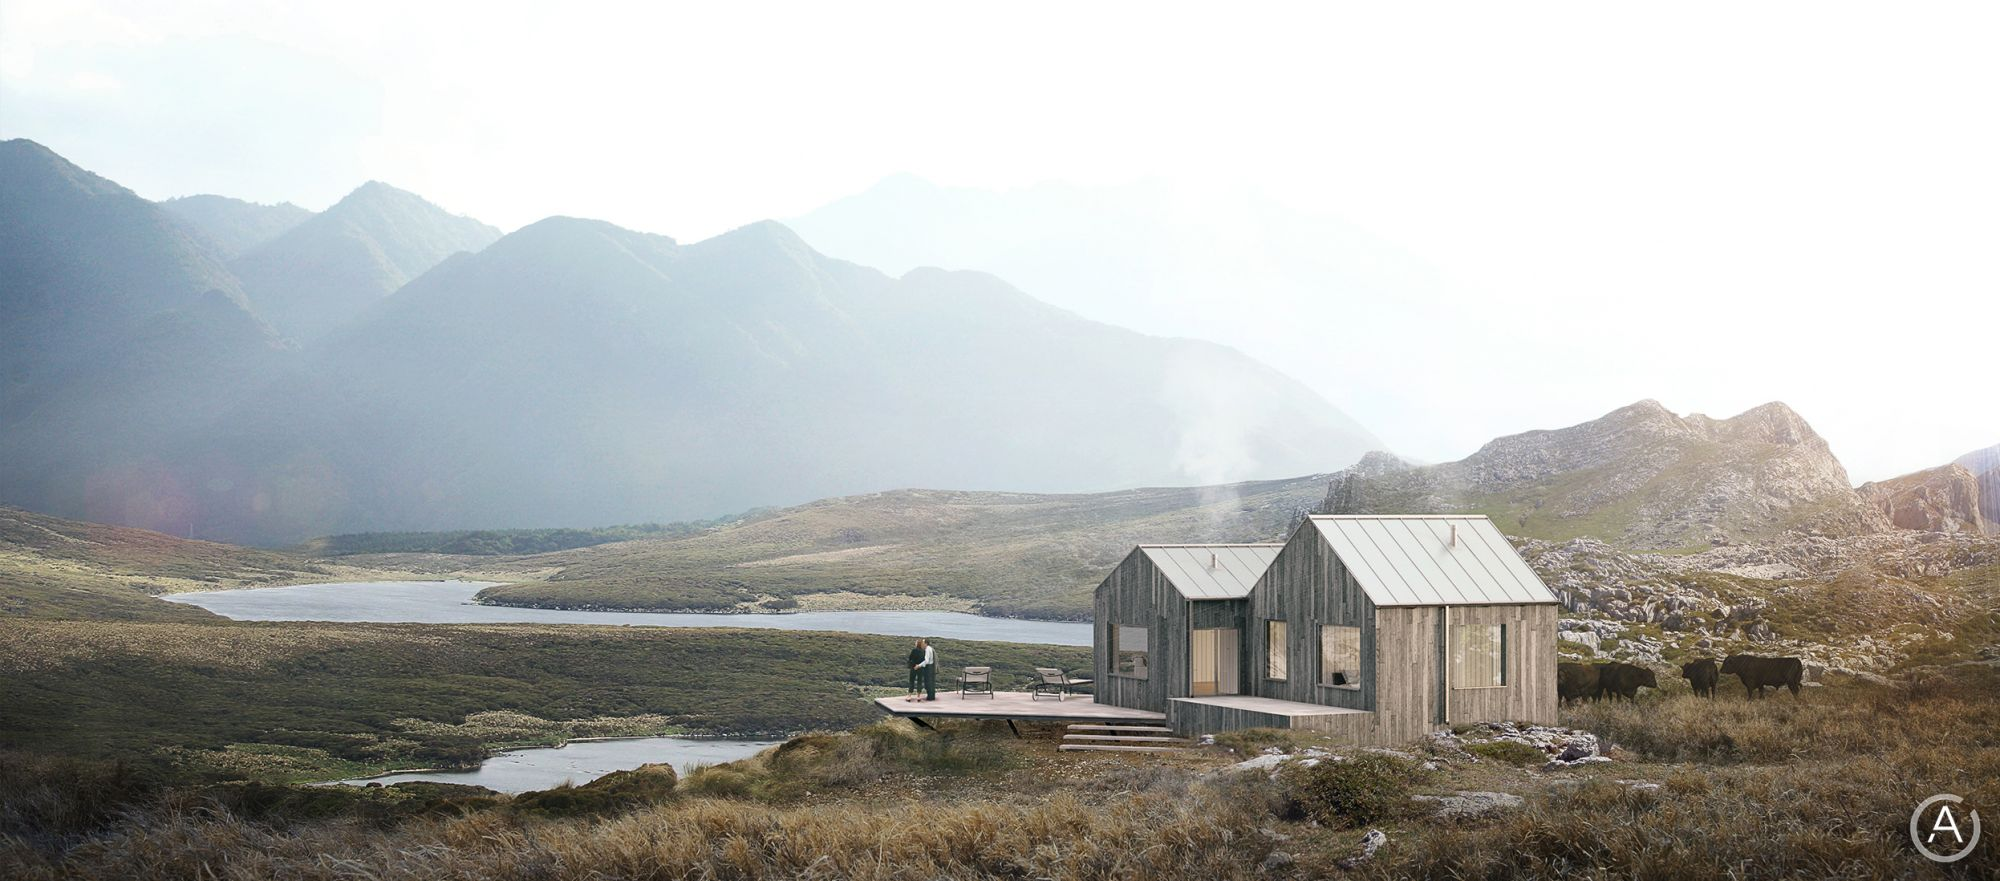
\includegraphics[height=6cm]{img/cabana_01_large.jpg}
	\caption{TEST Image}
	\label{fig:lightingtypes}
\end{figure}
\end{frame}
\begin{center}\line(1,0){250}\end{center}


\section{Color Temperature}

\begin{frame}
\frametitle{Color Temperature}
\begin{itemize}
	\item Color Temperature refers to the color cast generated by various types of lighting
	\item In digital photography it is often referred to as 'White Balance'.
	\item Incandecent lamps tend to project warm colors; LED and florescent lamps tend to have a cold cast.
	\item The color temperature scale is Kelvin
	\item Lower color temps are warm, higher color temps are cold
\end{itemize}
\end{frame}
\begin{center}\line(1,0){250}\end{center}

\begin{frame}
\frametitle{Color Temperature}
\begin{itemize}
	\item 5000K is fairly neutral
	\item Incandescent lamps are about 3000K
	\item Florescent lamps can be about 6000K
\end{itemize}
\end{frame}
\begin{center}\line(1,0){250}\end{center}



\begin{frame}
\frametitle{3000 Kelvin}
\begin{figure}
	\centering
		\includegraphics[height=6cm]{img/3000K.png}
	\caption{3000K}
	\label{fig:colortemp3000}
\end{figure}
\end{frame}
\begin{center}\line(1,0){250}\end{center}


\begin{frame}
\frametitle{5000 Kelvin}
\begin{figure}
	\centering
		\includegraphics[height=6cm]{img/5000K.png}
	\caption{5000K}
	\label{fig:colortemp5000}
\end{figure}
\end{frame}
\begin{center}\line(1,0){250}\end{center}

\begin{frame}
\frametitle{8000 Kelvin}
\begin{figure}
	\centering
		\includegraphics[height=6cm]{img/8000K.png}
	\caption{8000K}
	\label{fig:colortemp8000}
\end{figure}
\end{frame}
\begin{center}\line(1,0){250}\end{center}

\begin{frame}
\frametitle{15000 Kelvin}
\begin{figure}
	\centering
		\includegraphics[height=6cm]{img/15000K.png}
	\caption{15000K}
	\label{fig:colortemp15000}
\end{figure}
\end{frame}
\begin{center}\line(1,0){250}\end{center}

\begin{frame}
\frametitle{Color Temperature}
\begin{itemize}
	\item Generally it is not a good idea to stray too far from the 4800-5000K range
	\item We can warm up, or cool down a scene by adjusting the color temperature up or down by 1000K
	\item Too much adjustment will force an artificial look on your image.
\end{itemize}
\end{frame}
\begin{center}\line(1,0){250}\end{center}



\section{State Sets}

\begin{frame}
\frametitle{State Sets}
\begin{itemize}
	\item Max provides us with the option of saving our models in various 'States' within the .max file
	\item It is extremely useful for keeping small adjustments within the model
	\item 'Manage State Sets' is available under the 'quad' menu.
	\item In the following images, state sets were used to retain material assignments for color options.
\end{itemize}
\end{frame}
\begin{center}\line(1,0){250}\end{center}


\begin{frame}
\frametitle{Base State}
\begin{figure}
	\centering
		\includegraphics[height=6cm]{img/Base.png}
	\caption{Base State}
	\label{fig:BaseState}
\end{figure}
\end{frame}
\begin{center}\line(1,0){250}\end{center}

\begin{frame}
\frametitle{Yellow Paint}
\begin{figure}
	\centering
		\includegraphics[height=6cm]{img/yellow.png}
	\caption{Yellow State Set}
	\label{fig:yellow}
\end{figure}
\end{frame}
\begin{center}\line(1,0){250}\end{center}

\begin{frame}
\frametitle{Red Paint}
\begin{figure}
	\centering
		\includegraphics[height=6cm]{img/red.png}
	\caption{RedPaint State Set}
	\label{fig:RedPaint}
\end{figure}
\end{frame}
\begin{center}\line(1,0){250}\end{center}

\begin{frame}
\frametitle{Olive Green Paint}
\begin{figure}
	\centering
		\includegraphics[height=6cm]{img/OliveGreen.png}
	\caption{OliveGreen State Set}
	\label{fig:OliveGreen}
\end{figure}
\end{frame}
\begin{center}\line(1,0){250}\end{center}


\begin{frame}
\frametitle{State Sets}
\begin{itemize}
	\item State sets are not limited to simple material changes
	\item Cameras, Materials, Geometery, Lights, and other scene attributes can be saved in a state set
	\item Used correctly state sets can greatly improve the speed of your workflow, and can be used for batch rendering.
\end{itemize}
\end{frame}
\begin{center}\line(1,0){250}\end{center}

\section{Rendering Engines}
\begin{frame}
\title[Rendering Engines]{Rendering Engines}
\titlepage
\end{frame}\begin{center}\line(1,0){250}\end{center}

\begin{frame}
\frametitle{Rendering Engines}
Max ships with a number of rendering engines
\begin{itemize}
	\item \textbf{Scanline} - poor quality, fast, good for checks, but not recommended
	\item \textbf{ART} - better but still not recommended
	\item \textbf{Mental Ray} - NVIDIA product, appropriate for production
	\item \textbf{IRay} - NVIDIA product, was set to replace Mental Ray; but wont.
	\item \textbf{Quicksilver} - Hardware Renderer - fast, quality good
	\item \textbf{Arnold} - Autodesk product, can't make it work
	\item \textbf{V-Ray} - Go-to production renderer for ArchViz
\end{itemize}
\end{frame}
\begin{center}\line(1,0){250}\end{center}



\begin{frame}
\frametitle{Scanline Image}
\begin{figure}
	\centering
		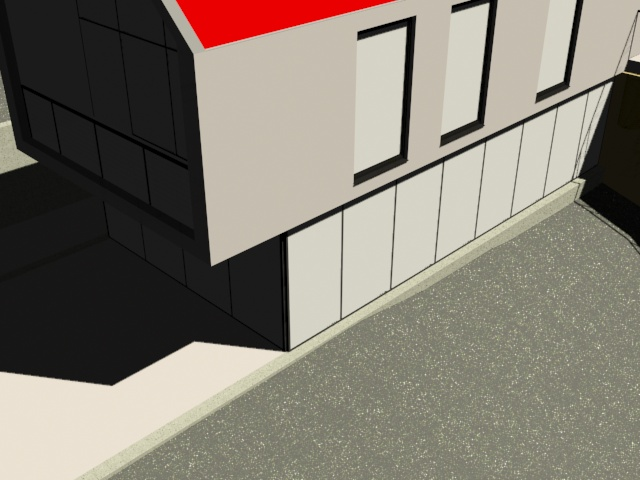
\includegraphics[height=6cm]{img/RenderEngine/Revit3DSScanLine.jpg}
	\caption{Scanline Renderer}
	\label{fig:Scanline}
\end{figure}
\end{frame}
\begin{center}\line(1,0){250}\end{center}


\begin{frame}
\frametitle{ART Renderer Image}
\begin{figure}
	\centering
	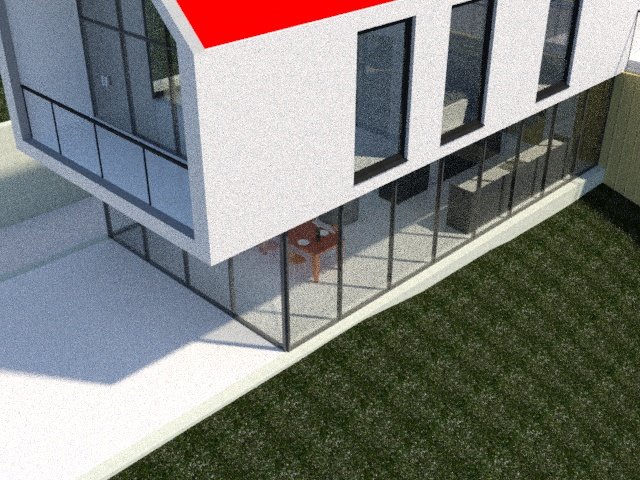
\includegraphics[height=6cm]{img/RenderEngine/Revit3DSARTRenderer.jpg}
	\caption{Scanline Renderer}
	\label{fig:Scanline}
\end{figure}
\end{frame}
\begin{center}\line(1,0){250}\end{center}






\begin{frame}
\frametitle{Mental Ray Image}
\begin{figure}
	\centering
		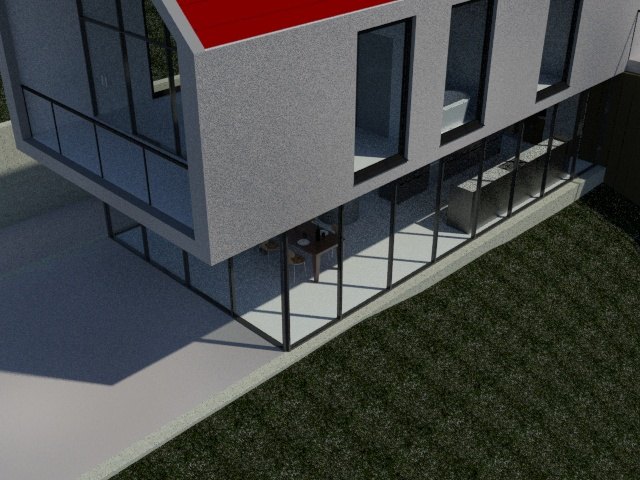
\includegraphics[height=6cm]{img/RenderEngine/Revit3DSMentalRay.jpg}
	\caption{Mental Ray Renderer}
	\label{fig:MentalRay}
\end{figure}
\end{frame}
\begin{center}\line(1,0){250}\end{center}



\begin{frame}
\frametitle{IRay image}
\begin{figure}
	\centering
		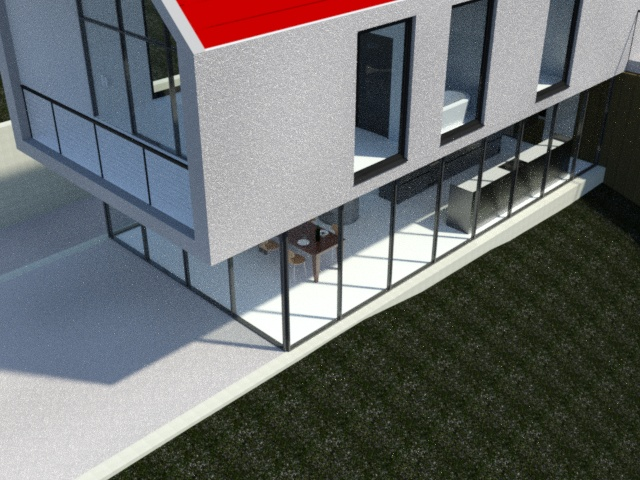
\includegraphics[height=6cm]{img/RenderEngine/Revit3DSIRay.jpg}
	\caption{IRay - note grey panel behind red vase}
	\label{fig:IRay}
\end{figure}
\end{frame}
\begin{center}\line(1,0){250}\end{center}


\begin{frame}
\frametitle{Quicksilver Hardware Renderer}
\begin{figure}
	\centering
	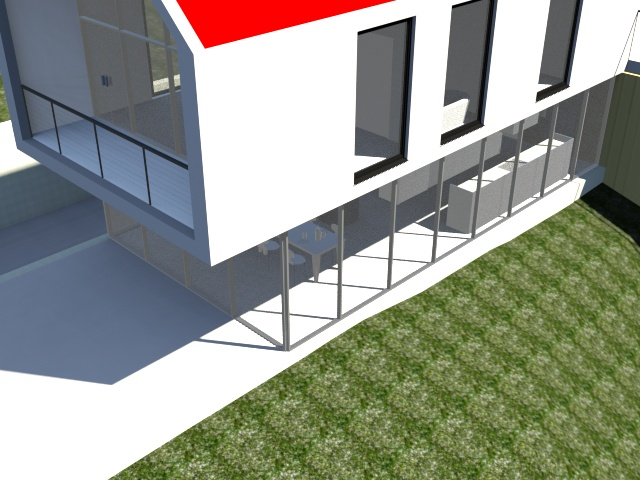
\includegraphics[height=6cm]{img/RenderEngine/Revit3DSQuickSilver.jpg}
	\caption{Scanline Renderer}
	\label{fig:Scanline}
\end{figure}
\end{frame}
\begin{center}\line(1,0){250}\end{center}


\begin{frame}
\frametitle{Arnold Renderer}
\begin{figure}
	\centering
	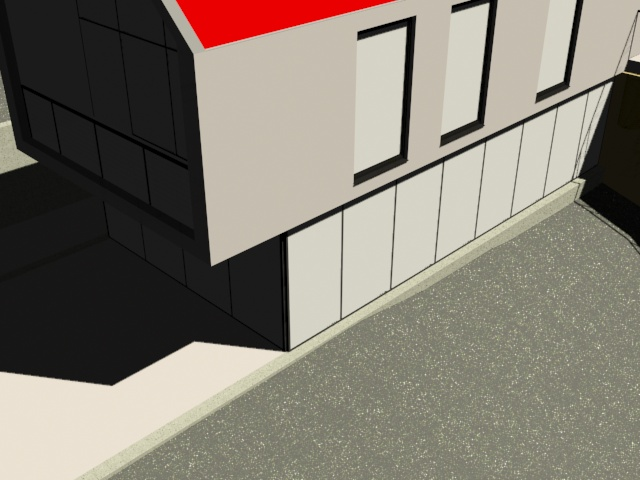
\includegraphics[height=6cm]{img/RenderEngine/Revit3DSScanLine.jpg}
	\caption{Scanline Renderer}
	\label{fig:Scanline}
\end{figure}
\end{frame}
\begin{center}\line(1,0){250}\end{center}

\begin{frame}
\frametitle{V-Ray Renderer}
\begin{figure}
	\centering
	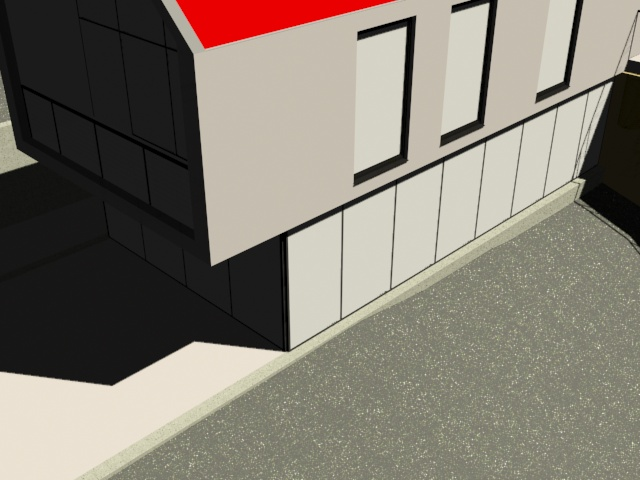
\includegraphics[height=6cm]{img/RenderEngine/Revit3DSScanLine.jpg}
	\caption{Scanline Renderer}
	\label{fig:Scanline}
\end{figure}
\end{frame}
\begin{center}\line(1,0){250}\end{center}




\begin{frame}
\frametitle{Rendering Engines and Materials}
\begin{itemize}
	\item Unfortunately, not all materials work with all rendering engines.
	\item Mental Ray supports features that IRAY does not.
	\item If IRAY cannot resolve a material correctly it will render it as gray.
\end{itemize}
\end{frame}
\begin{center}\line(1,0){250}\end{center}


\begin{frame}
\frametitle{Rendering Tweeks}
\begin{itemize}
	\item Ambient Occlusion - Mental Ray: adds soft shadows to small objects.  Adds richness to the image
	\item 
\end{itemize}
\end{frame}
\begin{center}\line(1,0){250}\end{center}





\section{Technology}


\begin{frame}
\frametitle{Rendering Engines}
3DS ships with two rendering engines
\begin{itemize}
	\item \textbf{Scanline:} Internal Autodesk, fast, generally poor quality, not recommended
	\item \textbf{Mental Ray:} by NVIDIA; better, good integration with 3DS.  Can use standard, autodesk or Mental Ray materials.  Good level of customization possible
\end{itemize}
Another Rendering Engine you will come across is \textbf{V-Ray}. This is the preferred option for most visualization houses due to its high levels of accuracy and third level support.  It is available to students at discounted rates; currently about \$200.00
\end{frame}
\begin{center}\line(1,0){250}\end{center}



\begin{frame}
\frametitle{Graphics Cards}
The graphics cards does most of the rendering work, and as such you need a good one to produce renders within a reasonable amount of time.  There are hundreds of graphics cards on the market, however you will find that most fall into one of two main options
\begin{itemize}
	\item NVIDIA
	\item Raytheon
\end{itemize}
Remember that NVIDIA is the creator of Mental Ray, so you will find that Mental Ray performs best with NVIDIA hardware.
\end{frame}
\begin{center}\line(1,0){250}\end{center}


\begin{frame}
\frametitle{Graphics Cards \hfill\hfill Things to watch for}
There are two main components of a graphics card that indicates its level of performance
\begin{itemize}
	\item Memory
	\item Number or graphics processors (GPUs)
\end{itemize}
Often people will select a card on memory alone; although important for CG work you also need more GPUs in order to crunch through the render calculations.  A good resource for comparing graphics cards is \href{http://www.videocardbenchmark.net/}{http://www.videocardbenchmark.net/}
\end{frame}
\begin{center}\line(1,0){250}\end{center}



\section{3D Printing}
\begin{frame}
\title[3D Printing]{3D Printing}
\titlepage
\end{frame}\begin{center}\line(1,0){250}\end{center}

\begin{frame}
\frametitle{3D Printing}
3D Printing is an additive technology.  What this means is that material is added to the component in order to create it.  This is different to many other technologies where material is removed to create a component.

\end{frame}
\begin{center}\line(1,0){250}\end{center}


\begin{frame}
\frametitle{3D Printing Applications}
\begin{figure}[h]
	\centering
	\includegraphics[height=6cm]{img/3DPrinting/3dprintedColumn.jpg}
	\caption[3D Printed Columns]{3D Printed Columns}
	\label{fig:3dprintcolumn}
\end{figure}
\end{frame}
\begin{center}\line(1,0){250}\end{center}


\begin{frame}
\frametitle{3D Printing Applications}
\begin{figure}[h]
	\centering
	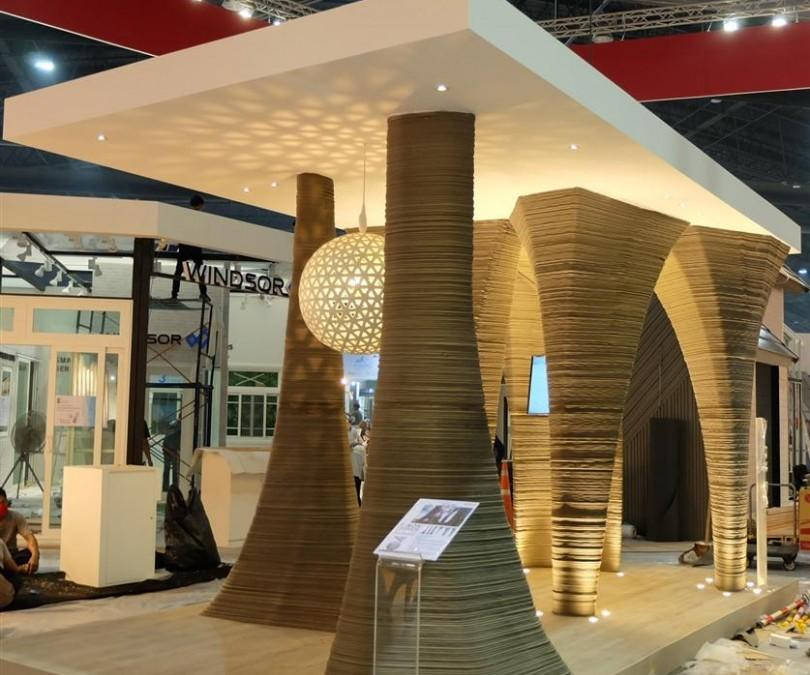
\includegraphics[height=6cm]{img/3DPrinting/3dprintColumn.jpg}
	\caption[3D Printed Columns]{3D Printed Columns}
	\label{fig:3dprintcolumn}
\end{figure}
\end{frame}
\begin{center}\line(1,0){250}\end{center}




\begin{frame}
\frametitle{3D Printing Applications}
\begin{figure}[h]
	\centering
	\includegraphics[height=6cm]{img/3DPrinting/3dprintedObject.jpg}
	\caption[3D Printed Object]{3D Printed Object}
	\label{fig:3dprintObject}
\end{figure}
\end{frame}
\begin{center}\line(1,0){250}\end{center}

\begin{frame}
\frametitle{3D Printing Applications}
\begin{figure}[h]
	\centering
	\includegraphics[height=6cm]{img/3DPrinting/3dprintFeature.jpg}
	\caption[3D Printed Feature]{3D Printed Feature}
	\label{fig:3dprintFeature}
\end{figure}
\end{frame}
\begin{center}\line(1,0){250}\end{center}


\begin{frame}
\frametitle{3D Printing Applications}
\begin{figure}[h]
	\centering
	\includegraphics[height=6cm]{img/3DPrinting/3dprintModel.jpg}
	\caption[3D Printed Model]{3D Printed Model}
	\label{fig:3dprintModel}
\end{figure}
\end{frame}
\begin{center}\line(1,0){250}\end{center}




\begin{frame}
\frametitle{Types of 3D Printer}
3D Printers exist for many types of materials and applications.  The choice of 3D print methodology will be dictated by:
\begin{itemize}
	\item Component Material
	\item Component Size
	\item Component finish (print resolution)
	\item Quantity required
	\item Turnaround Time
\end{itemize}

\end{frame}
\begin{center}\line(1,0){250}\end{center}

\begin{frame}
\frametitle{Types of 3D Printer}
Numerious types of printer exist, however the most common types are:
\begin{itemize}
	\item FDM - Fused Deposition Modelling
	\item SLS - Selective Layer Sintering
	\item SLA - Stereolithography
	\item DLP - Digital Light Projection
	\item Plaster Printer
\end{itemize}
\end{frame}
\begin{center}\line(1,0){250}\end{center}

\begin{frame}
\frametitle{FDM Printer}
Most common and affordable type of printer.  The main parts are the print bed and the extruder.  Both items move in order to put down a layer of material on the bed. The bed is then lowered for the next layer of material to be placed on top.  Only material needed to create the model, and its supporting structure, is used.  Resolution is typically 0.25mm
\end{frame}
\begin{center}\line(1,0){250}\end{center}



\begin{frame}
\frametitle{SLS Printer}
An SLS printer puts down an entire layer of material poweder, typically nylon.  The poweder layer is then fused by a laser into the shape needed for each layer.  Unused, or unfused powder can be recovered and used for the next print.  The final object often needs cleaning once complete.  Resolution of 0.1mm are typical.  These printers are very expensive, and are often used by specialist 3D print bureaus.
\end{frame}
\begin{center}\line(1,0){250}\end{center}


\begin{frame}
\frametitle{SLA/DLP Printers}
SLA and DLP Printers use a liquid resin as opposed to a solid or powder medium.  Parts are typically pulled out of a resin bath in an upward direction.  A layer fires from below to cure the resin into the desired layer shape.  The print resolution is very fine, better than 0.1mm, as the material is liquid before curing.\\
The difference between SLA and DLP is down to the curing mechanism.  SLA printers use a laser to draw out the shape of the layer.  DLP printers use digital imaging technology to fire the entire layer at once.

\end{frame}
\begin{center}\line(1,0){250}\end{center}


\begin{frame}
\frametitle{Plaster Printers}
Similar to SLS printers, a full layer of powder material is laid down.  However in the case of a plaster printer a binding agent is used to create the solid.  Color can be achieved by adding color (CMYK) to the binding agent.  Like SLS printers, they can achieve high resolutions.
\end{frame}
\begin{center}\line(1,0){250}\end{center}


\begin{frame}
\frametitle{FDM Printer Filaments}
There are two main filaments used by FDM Printers:
\begin{itemize}
	\item PLA - Polylactic Acid
	\item ABS - Acrylonitrile Butadiene Styrene
\end{itemize}
PLA is the easiest and cheapest to use.  PLA is available in the studio in a number of colors. 
\end{frame}
\begin{center}\line(1,0){250}\end{center}

\begin{frame}
\frametitle{Printing with PLA}
PLA is the easiest to print with.  The following applies to the RS Pro IdeaWerk printer in the lab and should be your starting point when printing.
\begin{itemize}
	\item Extruder Temperature set to 215$^o$C
	\item Bed Temperature set to 25$^o$C
	\item For large prints, set Bed Temperature to 65$^o$C
\end{itemize}
PLA is biodegradable, and does not smell too bad during printing.
\end{frame}
\begin{center}\line(1,0){250}\end{center}


\begin{frame}
\frametitle{Printing with ABS}
We to not currently have ABS in stock.  Generally, ABS requires higher temperatures than PLA.
\begin{itemize}
	\item Extruder temperature should be  235$^o$C
	\item Bed temperature should be 115$^o$C
\end{itemize}
ABS is NOT biodegradable and creates a strong smell when printing.  ABS is not recommended for use in the studio.  If you have an application that requires ABS, please consult me.
\end{frame}
\begin{center}\line(1,0){250}\end{center}


\begin{frame}
\frametitle{Print Failures}
Prints fail quite frequently.  Knowing the failure mechanism can help to determine the fix:
\begin{itemize}
	\item Print does not stick to bed or falls over - Bed Temperature too low
	\item Layers do not stick together - Bed temp too low, or bed set too far away from extruder.
	\item Filament builds up on extruder head - Bed too close to extruder
	\item Print quality good at start, but gets poorer as the print progresses - Printer on unstable surface, or print too tall.
\end{itemize}
There are many more ways for prints to fail, but these tend to be the most common.  Before tinkering with the printer, always run a test print on a WTK file that you know works.
\end{frame}
\begin{center}\line(1,0){250}\end{center}



\begin{frame}
\frametitle{Printing Tips (PLA)}
\begin{itemize}
	\item Always use a Raft
	\item Choose a print orientation that will minimize overhangs during printing
	\item If you have overhangs, use a support
	\item Keep important finishes off the raft, and keep them unsupported where possible
\end{itemize}
\end{frame}
\begin{center}\line(1,0){250}\end{center}


\begin{frame}
\frametitle{Final Finish for Prints}
Spending time on the final finish can greatly enhance the impact of a 3D printed object.
\begin{itemize}
	\item It is possible to solder (with PLA) individual parts, but an adhesive is easier. Cyanoacrylate works well. 
	\item Always trim and sand off excess material, and locations were support or raft has been removed.
	\item Polish with a buffing wheel or similar
	\item PLA works well with acrylic paints.
\end{itemize}
\end{frame}
\begin{center}\line(1,0){250}\end{center}


\begin{frame}
\frametitle{Instructions for RS Pro IdeaWerk}
\begin{itemize}
	\item Create Model in 3DS or similar
	\item Export Model as '.stl' file
	\item Import Model to DoraWare
	\item Position, Scale and Set Print Parameters
	\item Generate GCode in Doraware
	\item Export WTK file to disk or USB.
\end{itemize}
\end{frame}
\begin{center}\line(1,0){250}\end{center}


\begin{frame}
\frametitle{Instructions for RS Pro IdeaWerk}
\begin{itemize}
	\item Put WTK file into a folder named '3DMODEL' on USB Drive
	\item Insert USB into 3D printer. Use touchscreen interface on printer to select WTK file.
	\item Press 'Print' on 3D printer.
	\item DO NOT LEAVE PRINTER UNATTENDED.
\end{itemize}
\end{frame}
\begin{center}\line(1,0){250}\end{center}





\section{Materials \& Shaders}
\begin{frame}
\title[Materials \& Shaders]{Materials \& Shaders}
\titlepage
\end{frame}\begin{center}\line(1,0){250}\end{center}

Materials are linked to rendering engine

Materials are one of the most difficult and rewarding aspects of digital visualisations.

Materials Libraries


Material
Shader
Texture

Procedural Materials
Mapped Materials

Standard Materials

Special Materials








\section{Rendering}
\begin{frame}
\title[Rendering]{Rendering}
\titlepage
\end{frame}\begin{center}\line(1,0){250}\end{center}


\section{Project Setup}
\begin{frame}
\title[Project Setup]{Project Setup}
\titlepage
\end{frame}\begin{center}\line(1,0){250}\end{center}








\newpage

%
%This is some text 


\bibliographystyle{plainnat}
%\bibliographystyle{Classes/CUEDbiblio}
%\bibliographystyle{Classes/jmb}
%\bibliographystyle{Classes/jmb} % bibliography style
\nocite{*}
%\renewcommand{\bibname}{Bibliography} % changes default name References to Bibliography
\addcontentsline{toc}{chapter}{Bibliography}

\bibliography{refs/references} % References file

\newpage

\printindex
\newpage





\end{document}
